\documentclass[12pt]{report}
\usepackage[letterpaper]{geometry}
\geometry{verbose,tmargin=1.25in,bmargin=1.25in,lmargin=1.4in,rmargin=1.15in}
\usepackage[doublespacing]{setspace}
\usepackage{tocloft}
\usepackage[rm, tiny, center, compact]{titlesec}
\usepackage{indentfirst}
\usepackage{etoolbox}
\usepackage{tocvsec2}
\usepackage[titletoc]{appendix}
\usepackage{appendix}
\usepackage{longtable}  % for tables that are too large for a single page
\usepackage{tamuconfig}
\usepackage{rotating}   % to allow rotation of floats
\usepackage{color}
\usepackage{xcolor}
\usepackage{alltt}
\usepackage{amsmath}
\usepackage{amssymb}
\usepackage{empheq} % for emphasizing certain equations
\usepackage{booktabs}
\usepackage{subcaption}
\usepackage[mathscr]{euscript} % for \mathscr{} in math mode
\usepackage[hidelinks]{hyperref}

% input user-defined commands
% required packages
\usepackage{xcolor}
\usepackage{stmaryrd} % jump brackets: \llbracket, \rrbracket

% create a provideenvironment command
\makeatletter
\def\provideenvironment{\@star@or@long\provide@environment}
\def\provide@environment#1{%
  \@ifundefined{#1}%
    {\def\reserved@a{\newenvironment{#1}}}%
    {\def\reserved@a{\renewenvironment{dummy@environ}}}%
  \reserved@a
}
\def\dummy@environ{}
\makeatother

% directories
\newcommand{\diagramdirectory}{../diagrams}

% general
\newcommand{\x}{\mathbf{x}}
\newcommand{\qpoint}{\x_q}
\newcommand{\timevalue}{t}
\newcommand{\timestepsize}{\Delta\timevalue}
\newcommand{\dt}{\timestepsize}
\newcommand{\timeindex}{n}
\newcommand{\speed}{v}
\newcommand{\velocity}{\mathbf{\speed}}
\newcommand{\velocityx}{u}
\newcommand{\velocityy}{v}
\newcommand{\velocityn}{v_n}
\newcommand{\vx}{\velocityx}
\newcommand{\vy}{\velocityy}
\newcommand{\vn}{\velocityn}

% normal vector
\newcommand{\normalvectorletter}{n}
\newcommand{\normalvector}{\mathbf{\normalvectorletter}}
\newcommand{\normalx}{\normalvectorletter_x}
\newcommand{\normaly}{\normalvectorletter_y}
\newcommand{\nx}{\normalx}
\newcommand{\ny}{\normaly}

\newcommand{\ndimensions}{N_\text{dim}}
\newcommand{\ncomponents}{m}
\newcommand{\ndofs}{N_\text{dof}}
\newcommand{\nnodes}{N_\text{node}}
\newcommand{\dofindex}{j}
\newcommand{\nodeindex}{k}
\newcommand{\componentindex}{k}
\newcommand{\transpose}{^{\text{T}}}

% schemes
\newcommand{\low}{L}
\newcommand{\high}{H}

% solution
\newcommand{\scalarsolution}{u}
\newcommand{\vectorsolution}{\mathbf{\scalarsolution}}
\newcommand{\approximate}[1]{\tilde{#1}}
\newcommand{\approximatescalarsolution}{\approximate{\scalarsolution}}
\newcommand{\approximatevectorsolution}{\approximate{\vectorsolution}}
\newcommand{\solutionletter}{U}
\newcommand{\solutionvector}{\mathbf{\solutionletter}}
\newcommand{\U}{\solutionvector}
\newcommand{\lowordersolution}[1][]{
  \ifthenelse{\equal{#1}{}}{\solutionvector^L}{\solutionvector^{L,#1}}}
\newcommand{\highordersolution}[1][]{
  \ifthenelse{\equal{#1}{}}{\solutionvector^H}{\solutionvector^{H,#1}}}

% math
\newcommand{\triangulation}{\mathcal{K}_h}
\newcommand{\approximationspace}{\mathcal{U}_h}
\newcommand{\approximationspaceinc}{\approximationspace^{\textup{inc}}}
\newcommand{\referenceelementmap}{\Phi}
\newcommand{\qonespace}{\mathbb{Q}_1}

% sets
\newcommand{\faces}{\mathcal{F}}
\newcommand{\quadraturepoints}{\mathcal{Q}}

% domain and FEM
\newcommand{\domain}{\mathcal{D}}
\newcommand{\celldomain}[1][\cell]{\domain_#1}
\newcommand{\facedomain}{\domain}
\newcommand{\domainboundary}{\partial\domain}
\newcommand{\incomingdomainboundary}{\domainboundary^{\textup{inc}}}
\newcommand{\cellindex}{K}
\newcommand{\cell}{K}
\newcommand{\celldiameter}{\Delta x}
\newcommand{\maxcelldiameter}{\Delta x_{\text{max}}}
\newcommand{\volume}{V}
\newcommand{\dvolume}{\,d\x}
\newcommand{\area}{A}
\newcommand{\darea}{\,d\area}
\newcommand{\testfunction}{\varphi}
\newcommand{\vectortestfunctionscalar}{\Phi}
\newcommand{\vectortestfunction}{\mathbf{\vectortestfunctionscalar}}
\newcommand{\support}{S}
\newcommand{\maxdof}{N}
\newcommand{\interpolant}{\Pi}

% local viscous bilinear form
\newcommand{\localvisc}{b}
\newcommand{\localviscbilinearform}[3]{\localvisc_#1(\testfunction_#2, \testfunction_#3)}
\newcommand{\cellvolume}{|\celldomain|}
\newcommand{\cardinality}[1][]{\ifthenelse{\equal{#1}{}}{n_\cell}{n_#1}}
\newcommand{\cardsystem}{\bar{n}}
\newcommand{\indices}{\mathcal{I}}
\newcommand{\cellindices}{\mathcal{K}}
\newcommand{\indicesnode}{\indices^{\text{node}}_\cell}
\newcommand{\indicescell}[1][]{\ifthenelse{\equal{#1}{}}{\indices_\cell}
  {\indices_{#1}}}
\newcommand{\incomingindices}{\indices^{\textup{inc}}}
\newcommand{\notincomingindices}{\indices(\triangulation)\setminus\incomingindices}

% entropy viscosity
\newcommand{\entropy}{\eta}
\newcommand{\entropyflux}{\mathbf{\consfluxletter}^\eta}
\newcommand{\entropyjump}{\mathcal{J}}
\newcommand{\entropyresidual}{\mathcal{R}}
\newcommand{\entropyresidualcoef}{c_\entropyresidual}
\newcommand{\entropyjumpcoef}{c_\entropyjump}
\newcommand{\entropynormalization}{\hat{\entropy}}

% conservation law
\newcommand{\consfluxletter}{f}
\newcommand{\consflux}{\mathbf{\consfluxletter}}
\newcommand{\consfluxsystem}{\mathbf{\MakeUppercase{\consfluxletter}}}
\newcommand{\consfluxscalar}[1][\scalarsolution]{\mathbf{\consfluxletter}(#1)}
\newcommand{\consfluxvector}{\mathbf{\MakeUppercase{\consfluxletter}}}
\newcommand{\consfluxvectory}{\mathbf{G}}
\newcommand{\consfluxvectorn}{\consfluxvector_{n}}
\newcommand{\consfluxinterpolant}{\mathrm{F}}
\newcommand{\conssource}{\mathbf{s}}

% viscosity
\newcommand{\viscosity}{\nu}
\newcommand{\cellviscosity}{\viscosity_\cellindex}
\newcommand{\lowordercellviscosity}[1][]{
  \ifthenelse{\equal{#1}{}}{\cellviscosity^L}
  {\cellviscosity^{L,#1}}}
\newcommand{\highordercellviscosity}[1][]{
  \ifthenelse{\equal{#1}{}}{\cellviscosity^H}
  {\cellviscosity^{H,#1}}}
\newcommand{\entropycellviscosity}[1][]{
  \ifthenelse{\equal{#1}{}}{\cellviscosity^\entropy}
  {\cellviscosity^{\entropy,#1}}}

% viscous fluxes
\newcommand{\viscstring}{\text{visc}}
\newcommand{\viscflux}[1]{\mathbf{\consfluxletter}^{\viscstring,#1}}
\newcommand{\viscconsfluxvector}
  {\mathbf{\MakeUppercase{\consfluxletter}}^\viscstring
  (\vectorsolution,\viscosity)}

% mass matrix
\newcommand{\massmatrixletter}{M}
\newcommand{\massmatrix}{\mathbf{\massmatrixletter}}
\newcommand{\M}{\massmatrix}
\newcommand{\consistentmassmatrix}{\massmatrix^C}
\newcommand{\consistentmassentry}{\massmatrixletter^C_{i,j}}
\newcommand{\lumpedmassmatrix}{\massmatrix^L}
\newcommand{\lumpedmassentry}{\massmatrixletter^L_{i,i}}

% gradient matrix (for conservation law systems)
\newcommand{\gradientmatrixletter}{c}
\newcommand{\gradientmatrix}{\mathbf{\MakeUppercase{\gradientmatrixletter}}}
\newcommand{\gradiententry}{\mathbf{\gradientmatrixletter}\ij}

% steady-state system matrix and rhs
\newcommand{\ssmatrixletter}{A}
\newcommand{\ssmatrix}[1][]{
  \ifthenelse{\equal{#1}{}}
  {\mathbf{\ssmatrixletter}}
  {\mathbf{\ssmatrixletter}^#1}}
\newcommand{\A}{\ssmatrix}
\newcommand{\loworderssmatrix}[1][]{
  \ifthenelse{\equal{#1}{}}
  {\ssmatrix^L}
  {\ssmatrix^{L,#1}}}
\newcommand{\highorderssmatrix}[1][]{
  \ifthenelse{\equal{#1}{}}
  {\ssmatrix^H}
  {\ssmatrix^{H,#1}}}
\newcommand{\ssrhsletter}{b}
\newcommand{\ssrhs}[1][]{
  \ifthenelse{\equal{#1}{}}
  {\mathbf{\ssrhsletter}}
  {\mathbf{\ssrhsletter}^#1}}
\renewcommand{\b}{\ssrhs}
\newcommand{\ssresletter}{r}
\newcommand{\ssres}{\mathbf{\ssresletter}}
\renewcommand{\r}{\ssres}
\newcommand{\B}{\mathbf{B}}
\newcommand{\s}{\mathbf{s}}

% diffusion matrix
\newcommand{\diffusionmatrixletter}{D}
\newcommand{\diffusionmatrix}[1][]{
  \ifthenelse{\equal{#1}{}}
  {\mathbf{\diffusionmatrixletter}}
  {\mathbf{\diffusionmatrixletter}^#1}}
\newcommand{\D}{\diffusionmatrix}
\newcommand{\loworderdiffusionmatrix}[1][]{
  \ifthenelse{\equal{#1}{}}
  {\diffusionmatrix^L}
  {\diffusionmatrix^{L,#1}}}
\newcommand{\highorderdiffusionmatrix}[1][]{
  \ifthenelse{\equal{#1}{}}
  {\diffusionmatrix^H}
  {\diffusionmatrix^{H,#1}}}

% Runge-Kutta
\newcommand{\RKstagesolution}{\hat{\mathbf{\solutionletter}}}
\newcommand{\RKintermediatesolution}{\tilde{\mathbf{\solutionletter}}}
\newcommand{\RKoldsolutioncoef}{\alpha}
\newcommand{\RKstagesolutioncoef}{\beta}
\newcommand{\RKtimecoef}{c}
\newcommand{\RKstagetime}{\hat{\timevalue}}
\newcommand{\RKnstages}{s}

% FCT
\newcommand{\solutionbound}{W}
\newcommand{\DMPlowerbound}{\solutionbound^{\textup{DMP},-}}
\newcommand{\DMPupperbound}{\solutionbound^{\textup{DMP},+}}
\newcommand{\DMPlowerboundss}{\solutionbound^{\textup{DMP},\textup{ss},-}}
\newcommand{\DMPupperboundss}{\solutionbound^{\textup{DMP},\textup{ss},+}}
\newcommand{\DMPboundsss}{\solutionbound^{\textup{DMP},\textup{ss},\pm}}
\newcommand{\DMPlowerboundee}{\solutionbound^{\textup{DMP},\textup{ee},-}}
\newcommand{\DMPupperboundee}{\solutionbound^{\textup{DMP},\textup{ee},+}}
\newcommand{\DMPboundsee}{\solutionbound^{\textup{DMP},\textup{ee},\pm}}
\newcommand{\DMPlowerboundtheta}{\solutionbound^{\textup{DMP},\textup{theta},-}}
\newcommand{\DMPupperboundtheta}{\solutionbound^{\textup{DMP},\textup{theta},+}}
\newcommand{\DMPboundstheta}{\solutionbound^{\textup{DMP},\textup{theta},\pm}}
\newcommand{\DMPbounds}{\solutionbound^{\textup{DMP},\pm}}
\newcommand{\analyticDMPbounds}{\solutionbound^{\textup{analytic},\pm}}
\newcommand{\analyticDMPupperbound}{\solutionbound^{\textup{analytic},+}}
\newcommand{\analyticDMPlowerbound}{\solutionbound^{\textup{analytic},-}}
\newcommand{\limitedfluxbound}{Q}
\newcommand{\antidiffusionbound}{\limitedfluxbound}
\newcommand{\antidiffusionboundvector}{\mathbf{\limitedfluxbound}}
\newcommand{\antidiffusionlowerboundss}{\antidiffusionbound^{\textup{ss},-}}
\newcommand{\antidiffusionupperboundss}{\antidiffusionbound^{\textup{ss},+}}
\newcommand{\antidiffusionlowerboundee}{\antidiffusionbound^{\textup{ee},-}}
\newcommand{\antidiffusionupperboundee}{\antidiffusionbound^{\textup{ee},+}}
\newcommand{\antidiffusionlowerboundtheta}{\antidiffusionbound^{\textup{theta},-}}
\newcommand{\antidiffusionupperboundtheta}{\antidiffusionbound^{\textup{theta},+}}
\newcommand{\limitedfluxboundsi}{\limitedfluxbound^\pm_i}
\newcommand{\limiterletter}{L}
\newcommand{\limitermatrix}{\mathbf{\limiterletter}}
\newcommand{\correctionfluxletter}{p}
\newcommand{\correctionfluxvector}{\mathbf{\correctionfluxletter}}
\newcommand{\correctionfluxentry}{\MakeUppercase{\correctionfluxletter}}
\newcommand{\correctionfluxij}{\correctionfluxentry_{i,j}}
\newcommand{\correctionfluxji}{\correctionfluxentry_{j,i}}
\newcommand{\correctionfluxmatrix}{\mathbf{\MakeUppercase{\correctionfluxletter}}}
\newcommand{\antidiffusiveflux}{\correctionfluxentry}

% remainder
\newcommand{\correctionfluxremainder}{\Delta\MakeUppercase{\correctionfluxletter}}
\newcommand{\correctionfluxmatrixremainder}{\Delta\correctionfluxmatrix}
\newcommand{\limitedcorrectionfluxmatrixremainder}
  {\bar{\correctionfluxmatrixremainder}}

\newcommand{\limitedcorrectionfluxletter}{\bar{\correctionfluxletter}}
\newcommand{\cumulativecorrectionfluxletter}{\bar{\correctionfluxletter}}
\newcommand{\cumulativecorrectionfluxvector}{\bar{\correctionfluxvector}}
\newcommand{\cumulativecorrectionfluxvectorchange}
  {\Delta\cumulativecorrectionfluxvector}
\newcommand{\correctionfluxsumsi}{\MakeUppercase{\correctionfluxletter}^\pm_i}
\newcommand{\limitedfluxsum}{\limitermatrix\cdot\correctionfluxmatrix}
\newcommand{\limitedfluxsumi}{\sumj\limiterletter\ij
  \MakeUppercase{\correctionfluxletter}\ij}
\newcommand{\F}{\correctionfluxmatrix}
\newcommand{\LF}{\limitermatrix\cdot\correctionfluxmatrix}
\newcommand{\transformationmatrix}{\mathbf{T}}

% radiation transport
\newcommand{\angularflux}{\psi}
\newcommand{\scalarflux}{\phi}
\newcommand{\speedoflight}{c}
\newcommand{\totalcrosssection}{\Sigma_\text{t}}
\newcommand{\reactioncoef}{\sigma}
\newcommand{\directionvector}{\mathbf{\Omega}}
\newcommand{\di}{\directionvector}
\newcommand{\xdet}{(\x,\di,E,t)}
\newcommand{\xet}{(\x,E,t)}
\newcommand{\scalarsource}{q}
\newcommand{\radiationsource}{Q}

% Euler equations
\newcommand{\density}{\rho}
\newcommand{\totalenergy}{E}
\newcommand{\momentum}{\mathbf{m}}
\newcommand{\pressure}{p}
\newcommand{\gasconstant}{\gamma}
\newcommand{\identity}{\mathbf{I}}

% shallow water equations
\newcommand{\height}{h}
\newcommand{\heightmomentumletter}{q}
\newcommand{\heightmomentum}{\mathbf{\heightmomentumletter}}
\newcommand{\heightmomentumx}{\heightmomentumletter_x}
\newcommand{\heightmomentumy}{\heightmomentumletter_y}
\newcommand{\heightmomentumd}{\heightmomentumletter_d}
\newcommand{\dischargex}{\heightmomentumletter}
\newcommand{\bathymetry}{b}
\newcommand{\waterlevel}{w}
\newcommand{\gravity}{g}
\newcommand{\speedofsound}{a}
\newcommand{\froude}{\mathrm{Fr}}

% Riemann solvers
\newcommand{\shockspeed}{S}
\newcommand{\eigenvalue}{\lambda}
\newcommand{\eigenvaluematrix}{\mathbf{\Lambda}}
\newcommand{\eigenvector}{\mathbf{k}}
\newcommand{\eigenvectormatrix}{\mathbf{K}}
\newcommand{\jacobianx}{\mathbf{A}}
\newcommand{\jacobiany}{\mathbf{B}}
\newcommand{\jacobiann}{\jacobianx_{n}}
\newcommand{\characteristicsolution}{\mathbf{w}}
\newcommand{\wavespeed}{\eigenvalue}
\newcommand{\maxwavespeed}[1][]{
  \ifthenelse{\equal{#1}{}}{\wavespeed^{\text{max}}}{\wavespeed^{\text{max},#1}}}
\newcommand{\wavestrength}{\mathcal{W}}

%==============================================================================
% colors
\colorlet{lightBlue}{blue!20!white}
\colorlet{lightGreen}{green!20!white}

% indexing
\renewcommand{\ij}{_{i,j}}
\newcommand{\ji}{_{j,i}}
\newcommand{\kl}{_{k,\ell}}
\newcommand{\lk}{_{\ell,k}}
\newcommand{\nodei}{_{\nodeindex(i)}}
\newcommand{\nodej}{_{\nodeindex(j)}}
\newcommand{\nodeij}{_{\nodeindex(i),\nodeindex(j)}}
\newcommand{\nodeji}{_{\nodeindex(j),\nodeindex(i)}}
\newcommand{\nodequantity}[1]{\underline{#1}}

% sums and integrals
\newcommand{\sumj}{\sum\limits_j}
\newcommand{\sumjnoti}{\sum\limits_{j\ne i}}
\newcommand{\sumKSi}{\sum\limits_{\cell\in\cellindices(\support_i)}}
%\newcommand{\sumKSij}[1][\cell]
%  {\sum\limits_{#1:\celldomain[#1]\subset\support_{i,j}}}
\newcommand{\sumKSij}[1][\cell]
  {\sum\limits_{#1\in\cellindices(\support\ij)}}
\newcommand{\sumallcells}{\sum\limits_{\cell}}
\newcommand{\intdomain}[1]{\int\limits_\domain #1 \,\dvolume}
\newcommand{\intboundary}[1]{\int\limits_{\domainboundary} #1 \,d\area}
\newcommand{\intSi}{\int\limits_{\support_i}}
\newcommand{\intSij}{\int\limits_{\support_{i,j}}}

% math
\newcommand{\ltwonorm}[1]{\left\|#1\right\|_{L^2}} % L-2 norm

% BC
\newcommand{\interior}{^{\text{in}}}
\newcommand{\BC}{^{\text{BC}}}

% common fractions
\newcommand{\half}{\frac{1}{2}}
\newcommand{\fourth}{\frac{1}{4}}

% derivatives
\newcommand{\dd}[2]{\frac{d #1}{d #2}}               % ordinary derivative
\newcommand{\pd}[2]{\frac{\partial #1}{\partial #2}} % partial derivative
\newcommand{\ppt}[1]{\pd{#1}{t}}                     % partial d/dt
\newcommand{\ppx}[1]{\pd{#1}{x}}                     % partial d/dx
\newcommand{\ppy}[1]{\pd{#1}{y}}                     % partial d/dy
\newcommand{\ddt}[1]{\frac{d#1}{dt}}                 % ordinary d/dt

% typesetting
\newcommand{\pr}[1]{\left(#1\right)} % parentheses
\newcommand{\sq}[1]{\left[#1\right]} % square brackets
\newcommand{\jumpbrackets}[1]{\left\llbracket#1\right\rrbracket} % jump brackets
\newcommand{\tab}{\hspace*{0.5cm}}   % tab for verbatim evironments
\newcommand{\eqp}{\,.} % equation period
\newcommand{\eqc}{\,,} % equation comma

% miscellaneous
\newcommand{\xt}{\pr{\x,\timevalue}}
\newcommand{\divergence}{\nabla\cdot}
\newcommand{\unitvector}[1]{\hat{\mathbf{e}}_{#1}}

% command to highlight term in equation
\newcommand{\highlightblue}[1]{
  \colorbox{lightBlue}{$\displaystyle#1$}}
\newcommand{\highlightgreen}[1]{
  \colorbox{lightGreen}{$\displaystyle#1$}}

% QED symbol command
\providecommand{\qed}{\nobreak \ifvmode \relax \else
  \ifdim\lastskip<1.5em \hskip-\lastskip
  \hskip1.5em plus0em minus0.5em \fi \nobreak
  \vrule height0.75em width0.5em depth0.25em\fi}

% math environments
\provideenvironment{proof}[1][Proof]{\begin{trivlist}
\item[\hskip \labelsep {\bfseries #1}]}{\end{trivlist}}
\provideenvironment{example}[1][Example]{\begin{trivlist}
\item[\hskip \labelsep {\bfseries #1}]}{\end{trivlist}}
\newenvironment{remark}[1][Remark]{\begin{trivlist}
\item[\hskip \labelsep {\bfseries #1}]}{\end{trivlist}}

% table environment
% #1 = caption
% #2 = label
% #3 = table format (columns)
% #4 = header row
\newenvironment{mytable}[4]
  {\begin{table}[htb]\caption{#1\label{tab:#2}}\begin{center}
    \begin{tabular}
    {#3}\hline #4\\\hline}
  {\hline\end{tabular}\end{center}\end{table}}

% references commands
%\newcommand{\refsec}[1]{, \S#1}
\newcommand{\refsec}[1]{}

% algorithm shortcuts
\newcommand{\objective}{\phi}
\newcommand{\hmin}{\height_{\text{min}}}
\newcommand{\hmax}{\height_{\text{max}}}
\newcommand{\hlow}{\check{\height}}
\newcommand{\hhigh}{\hat{\height}}
\newcommand{\hrarefaction}{\tilde{\height}_*}
\newcommand{\tol}{\epsilon}
\newcommand{\minwavespeed}{\wavespeed_{\text{min}}}
\newcommand{\lowwavespeedone}{\check{\wavespeed}_1}
\newcommand{\highwavespeedone}{\hat{\wavespeed}_1}
\newcommand{\lowwavespeedtwo}{\check{\wavespeed}_2}
\newcommand{\highwavespeedtwo}{\hat{\wavespeed}_2}
\newcommand{\hinterplow}{\height_d}
\newcommand{\hinterphigh}{\height_u}

% checkboxes
\usepackage{amssymb}
\usepackage{xcolor}
\definecolor{myorangeheavy}{RGB}{255,150,0}
\newcommand{\checked}{
  \makebox[0pt][l]{$\square$}\raisebox{.15ex}
  {\hspace{0.1em}\textcolor{myorangeheavy}{$\checkmark$}}}
\newcommand{\unchecked}{
  \makebox[0pt][l]{$\square$}\hspace{0.9em}}

% highlighting
\newcommand{\hlorange}[1]{\textcolor{myorangeheavy}{#1}}

% invariant domains
\newcommand{\invariantset}{A}
\newcommand{\admissibleset}{\mathcal{A}}
\newcommand{\discreteprocess}{R}
\newcommand{\convexcoefficient}{a}
\newcommand{\convexelement}{\mathbf{b}}

% spaces
\newcommand{\realspace}[1][]{
  \ifthenelse{\equal{#1}{}}{\mathbb{R}}{\mathbb{R}^{#1}}}

% nonlinear solve
\newcommand{\nonlinearmatrix}{\mathbf{B}}
\newcommand{\nonlinearrhs}{\mathbf{s}}
\newcommand{\relaxationparameter}{\alpha}
\newcommand{\nonlineartolerance}{\epsilon}

% algorithm
\usepackage{algpseudocode}
\usepackage{algorithm}
\newcommand{\Break}{\State \textbf{break}}
\newcommand{\Not}{\textbf{not}\,}
\newcommand{\Error}[1]{\State \textbf{error}: #1}

% boundary conditions
\newcommand{\dirichlet}[1]{\tilde{#1}}

\newcommand{\rowsum}[1]{#1\mathbf{1}}

% convergence and error analysis
\newcommand{\order}{\mathcal{O}}
\newcommand{\err}{e}
\newcommand{\dx}{\Delta x}

% tolerance adjustment for line-breaking, to prevent \overfull warnings
\newenvironment{tolerant}[1]{
  \par\tolerance=#1\relax
}{
  \par
}

%==============================================================================
% Theorem environments for dissertation
%==============================================================================
\usepackage{ifthen}

\newtheorem{mytheorem}{Theorem}[section]
\newtheorem{mylemma}{Lemma}[section]
\newtheorem{mycorollary}{Corollary}[section]
\newtheorem{mydefinition}{Definition}[section]
\newtheorem{myproposition}{Proposition}[section]

\newenvironment{theorem}[2][]
   {\ifthenelse{\equal{#2}{}}{\begin{mytheorem}}
   {\begin{mytheorem}\textbf{\textup{(#2)}}}
   \ifthenelse{\equal{#1}{}}{}{\label{#1}}}
   {\end{mytheorem}}
\newenvironment{lemma}[2][]
   {\ifthenelse{\equal{#2}{}}{\begin{mylemma}}
   {\begin{mylemma}\textbf{\textup{(#2)}}}
   \ifthenelse{\equal{#1}{}}{}{\label{#1}}}
   {\end{mylemma}}
\newenvironment{corollary}[2][]
   {\ifthenelse{\equal{#2}{}}{\begin{mycorollary}}
   {\begin{mycorollary}\textbf{\textup{(#2)}}}
   \ifthenelse{\equal{#1}{}}{}{\label{#1}}}
   {\end{mycorollary}}
\newenvironment{definition}[2][]
   {\ifthenelse{\equal{#2}{}}{\begin{mydefinition}}
   {\begin{mydefinition}\textbf{\textup{(#2)}}}
   \ifthenelse{\equal{#1}{}}{}{\label{#1}}}
   {\end{mydefinition}}
\newenvironment{proposition}[2][]
   {\ifthenelse{\equal{#2}{}}{\begin{myproposition}}
   {\begin{myproposition}\textbf{\textup{(#2)}}}
   \ifthenelse{\equal{#1}{}}{}{\label{#1}}}
   {\end{myproposition}}



% create path to content directory
\newcommand{\contentdir}{content}

% create black bar where there are "Overfull"s
\overfullrule=1cm

%===============================================================================
% Document
%===============================================================================
\begin{document}

\renewcommand{\tamumanuscripttitle}{Solution of the Transport Equation Using
   Entropy Viscosity and the Flux-Corrected Transport Algorithm}
\renewcommand{\tamupapertype}{Dissertation}
\renewcommand{\tamufullname}{Joshua Edmund Hansel}
\renewcommand{\tamudegree}{Doctor of Philosophy}
\renewcommand{\tamuchairone}{Jean Ragusa}
\renewcommand{\tamumemberone}{Marvin Adams}
\newcommand{\tamumembertwo}{Jim Morel}
\newcommand{\tamumemberthree}{Jean-Luc Guermond}
\renewcommand{\tamudepthead}{Yassin Hassan}
\renewcommand{\tamugradmonth}{May}
\renewcommand{\tamugradyear}{2016}
\renewcommand{\tamudepartment}{Nuclear Engineering}

\providecommand{\tabularnewline}{\\}

\pagestyle{empty}
\pagenumbering{roman}

\begin{titlepage}
\begin{center}
\MakeUppercase{\tamumanuscripttitle}
\vspace{4em}

A \tamupapertype

by

\MakeUppercase{\tamufullname}

\vspace{4em}

\begin{singlespace}

Submitted to the Office of Graduate and Professional Studies of \\
Texas A\&M University \\

in partial fulfillment of the requirements for the degree of \\
\end{singlespace}

\MakeUppercase{\tamudegree}
\par\end{center}
\vspace{2em}
\begin{singlespace}
\begin{tabular}{ll}
 & \tabularnewline
& \cr
% If you have Co-Chairs comment out the 'Chair of Committee' line below and uncomment the 'Co-Chairs of Committee' line.
Chair of Committee, & \tamuchairone\tabularnewline
%Co-Chairs of Committee, & \tamuchairone\tabularnewline & \tamuchairtwo\tabularnewline
Committee Members, & \tamumemberone\tabularnewline
 & \tamumembertwo\tabularnewline
 & \tamumemberthree\tabularnewline
Head of Department, & \tamudepthead\tabularnewline

\end{tabular}
\end{singlespace}
\vspace{3em}

\begin{center}
\tamugradmonth \hspace{2pt} \tamugradyear

\vspace{3em}

Major Subject: \tamudepartment \par
\vspace{3em}
Copyright \tamugradyear \hspace{.5em}\tamufullname 
\par\end{center}
\end{titlepage}
\pagebreak{}





\begin{abstract}
The Flux-Corrected Transport (FCT) algorithm is
applied to the unsteady and steady-state particle transport equation. The proposed FCT method employs the following:
(1) a low-order, positivity-preserving scheme,
based on the application of M-matrix properties,
(2) a high-order scheme based on the entropy viscosity method introduced by
Guermond \cite{guermond_ev}, and
(3) local, discrete solution bounds derived from the integral transport equation.
The resulting scheme is second-order accurate in space,
enforces an entropy inequality, mitigates the formation of spurious
oscillations, and guarantees the absence of negativities.
Space discretization is achieved using  continuous finite elements. 
Time discretizations for unsteady problems include theta schemes
such as explicit and implicit Euler, and strong-stability preserving
Runge-Kutta (SSPRK) methods.
The developed scheme is shown to be robust with explicit time discretizations
but encounters nonlinear convergence difficulties for steady-state
and implicit time discretizations.
\end{abstract}

%%%%%%%%%%%%%%%%%%%%%%%%%%%%%%%%%%%%%%%%%%%%%%%%%%%%%%%%%%%%%%%%%%%%%%%
%%                           DEDICATION
%%%%%%%%%%%%%%%%%%%%%%%%%%%%%%%%%%%%%%%%%%%%%%%%%%%%%%%%%%%%%%%%%%%%%
\chapter*{DEDICATION}
% Needs to be set to part, so the TOC doesnt add 'CHAPTER ' prefix in the TOC.
\addcontentsline{toc}{chapter}{DEDICATION}  

%\indent
\vspace{3.5in}
\begin{center}To Siobh\'{a}n\end{center}

\pagebreak{}

\chapter*{ACKNOWLEDGMENTS}
% Needs to be set to part, so the TOC doesnt add 'CHAPTER ' prefix in the TOC.
\addcontentsline{toc}{chapter}{ACKNOWLEDGMENTS}  

\indent
First and foremost, I would like to thank my advisor, Dr. Jean Ragusa,
for his years of guidance, wisdom, patience, and expertise. I would also like to
thank Dr. Marco Delchini for his time, effort, and
knowledge in the development of methods for the shallow water equations.

I would like to thank Dr. Jean-Luc Guermond and Dr. Bojan Popov for their
time and expertise in entropy-based artificial dissipation and
conservation law methodology. Their recent work on discrete maximum principle-
preserving and invariant domain methods was the foundation of this dissertation.

I would like to thank all of those who have contributed to the
development of the \texttt{deal.II} finite element library, which has been
a tremendous help in the implementation of the methods given in this
dissertation. I would especially like to thank Dr. Wolfgang Bangerth
and Dr. Bruno Turcksin, who have quickly answered many questions I had regarding
the use of \texttt{deal.II}.

I would like to thank those who have contributed to the development
of FCT methods over the years, whose works were essential in the development
of the methodology used in this research. I would like to thank Dr. Dmitri Kuzmin
for his responses in my questions about FCT.

I would like to thank the the U.S. Department of Energy for providing
funding for this research through the Nuclear Energy University
Programs (NEUP) fellowship. I would also like to thank Dr. Richard
Martineau of Idaho National Laboratory for providing funding of
the last two semesters of research.

Lastly, I would like to thank my friends and family for their love and support.

\pagebreak{}

\chapter*{NOMENCLATURE}
\addcontentsline{toc}{chapter}{NOMENCLATURE}  

Table \ref{tab:abbreviations} lists the abbreviations used in this dissertation,
and Table \ref{tab:symbols} lists the symbols used in this dissertation.

\begin{mytable}{Abbreviations Used in Dissertation}{abbreviations}{l l}
{\emph{Abbreviation} & \emph{Description}}
DMP & discrete maximum principle\\
EV  & entropy viscosity\\
FCT & flux-corrected transport\\
FEM & finite element method\\
\end{mytable}

\begin{center}
\begin{longtable}{l p{4.8in}}
\caption{Symbols Used in Dissertation\label{tab:symbols}}\\
\hline
\emph{Symbol} & \emph{Description}\\
\hline
\endfirsthead
\hline
\emph{Symbol} & \emph{Description}\\
\hline
\endhead
\hline
\endfoot
\hline
\endlastfoot
%==============================================================================
% Latin alphabet: A-Z
%==============================================================================
% A-B
%------------------------------------------------------------------------------
$\ssmatrix$        & steady-state matrix\\
$\highorderssmatrix$ & high-order steady-state matrix\\
$\loworderssmatrix$ & low-order steady-state matrix\\
$\bathymetry$      & bathymetry (bottom topography) function for shallow
                     water equations\\
$\ssrhs$           & steady-state right hand side vector\\
$\localviscbilinearform_\cellindex(\testfunction_i,\testfunction_j)$ &
                     viscous bilinear form for cell $\cellindex$ and test
                     functions $\testfunction_i$ and $\testfunction_j$\\

% C
%------------------------------------------------------------------------------
$\speedoflight$    & speed of light\\
$\RKtimecoef_i$    & time step size fraction for stage $i$ of a
                     Runge-Kutta time step\\
$\entropyjumpcoef$ & coefficient for the entropy jump term in the definition
                     of entropy viscosity\\
$\entropyresidualcoef$ & coefficient for the entropy residual term in the
                         definition of entropy viscosity\\

% D
%------------------------------------------------------------------------------
$\highorderdiffusionmatrix$ & high-order diffusion matrix\\
$\loworderdiffusionmatrix$ & low-order diffusion matrix\\
$\domain$          & problem domain\\
$\domainboundary$  & problem domain boundary\\

% E-K
%------------------------------------------------------------------------------
$\totalenergy$     & total energy density\\
$\consfluxscalar$  & conservation law flux function for scalar case\\
$\consfluxvector$  & conservation law flux function for vector case\\
$\gravity$         & acceleration due to gravity\\
$\height$          & height\\
$\indicescell(\cellindex)$ & set of degree of freedom indices with support on
                             cell $\cellindex$\\
$\entropyjump_F$ & entropy jump for face $F$\\
$\cellindex$       & cell index\\

% L-M
%------------------------------------------------------------------------------
$\limitermatrix$   & matrix of limiting coefficients\\
$\limiterletter_{i,j}$ & limiting coefficient for degrees of freedom $i$
                         and $j$\\
$\limiterletter^\pm_i$ & limiting coefficient bounds for degree of freedom $i$
                         due to DMP of $i$ alone\\
$\momentum$        & momentum\\
$\consistentmassmatrix$ & consistent mass matrix\\
$\lumpedmassmatrix$ & lumped mass matrix\\

% N-P
%------------------------------------------------------------------------------
$\timeindex$       & time index\\
$\normalvector$    & normal vector to a surface\\
$\cardinalitycell$ & cardinality of cell $\cellindex$\\
$\pressure$        & pressure\\
$\correctionfluxvector$ & FCT correction flux vector\\
$\correctionfluxmatrix$ & matrix of FCT internodal correction flux entries\\
$\correctionfluxij$ & FCT internodal correction flux for degrees of freedom
                      $i$ and $j$\\
$\correctionfluxsumsi$ & sum of positive ($+$) and negative ($-$) FCT internodal
                         correction fluxes for degree of freedom $i$\\

% Q-T
%------------------------------------------------------------------------------
$\scalarsource$    & scalar source function\\
$\heightmomentum$  & ``momentum'' for shallow water equations,
                     $\height\velocity$\\
$\limitedfluxboundsi$ & upper and lower bounds for limited flux sum for degree
                        of freedom $i$\\
$\ssres$           & steady-state residual vector\\
$\entropyresidual_\cellindex$ & entropy residual for cell $\cellindex$\\
$\support_i$       & support of FEM test/basis function $i$\\
$\support\ij$      & dual support of FEM test/basis functions $i$ and $j$\\
$\conssource$      & conservation law source function\\
$\timevalue$       & time\\

% U
%------------------------------------------------------------------------------
$\RKstagetime_i$   & stage $i$ time of a Runge-Kutta time step\\
$\scalarsolution$  & depending on context, may denote either a scalar solution or
                     $x$ component of velocity\\
$\approximatescalarsolution$ & numerical approximation to $\scalarsolution$\\
$\solutionvector$  & solution vector\\
$\RKstagesolution^i$ & stage solution vector for stage $i$ of a Runge-Kutta time
                       step\\
$\RKintermediatesolution^i$ & intermediate solution vector for stage $i$ of a
                              Runge-Kutta time step\\
$\highordersolution$ & high-order solution vector\\
$\lowordersolution$ & low-order solution vector\\

% V-Z
%------------------------------------------------------------------------------
$\speed$           & speed\\
$\velocity$        & velocity\\
$\volume$          & volume\\
$\cellvolume$      & volume of cell $\cellindex$\\
$\DMPboundsi$      & upper and lower DMP bounds for degree of freedom $i$\\
$\x$               & spatial position\\
%==============================================================================
% Greek alphabet
%==============================================================================
% alpha - mu
%------------------------------------------------------------------------------
$\RKoldsolutioncoef_i$ & coefficient for the old solution vector in stage
                         $i$ of a Runge-Kutta time step\\
$\RKstagesolutioncoef_i$ & coefficient for the stage solution vector in stage
                           $i$ of a Runge-Kutta time step\\
$\timestepsize$    & time step size\\
$\entropy$         & entropy function\\
$\theta$           & parameter for $\theta$ time discretization scheme\\

% nu - omega
%------------------------------------------------------------------------------
$\lowordervisc$    & low-order viscosity for cell $\cellindex$\\
$\highordervisc$   & high-order viscosity for cell $\cellindex$\\
$\entropyvisc$     & entropy viscosity for cell $\cellindex$\\
$\density$         & density\\
$\reactioncoef$    & reaction coefficient\\
$\totalcrosssection$ & total macroscopic cross-section\\
$\testfunction$    & FEM test/basis function\\
$\angularflux$     & angular flux\\
$\directionvector$ & unit transport direction vector\\
%==============================================================================
\end{longtable}
\end{center}

\pagebreak{}

%%%%%%%%%%%%%%%%%%%%%%%%%%%%%%%%%%%%%%%%%%%%%%%%%%%
%
%  New template code for TAMU Theses and Dissertations starting Fall 2012.  
%  For more info about this template or the 
%  TAMU LaTeX User's Group, see http://www.howdy.me/.
%
%  Author: Wendy Lynn Turner 
%	 Version 1.4
%  Last updated 1/27/2013
%
%%%%%%%%%%%%%%%%%%%%%%%%%%%%%%%%%%%%%%%%%%%%%%%%%%%
%%%%%%%%%%%%%%%%%%%%%%%%%%%%%%%%%%%%%%%%%%%%%%%%%%%%%%%%%%%%%%%%%%%%%%
%%       TABLE OF CONTENTS
%%%%%%%%%%%%%%%%%%%%%%%%%%%%%%%%%%%%%%%%%%%%%%%%%%%%%%%%%%%%%%%%%%%%%
% single-space sections in Table of Contents
\renewcommand{\cftsecafterpnum}{\vskip0.5\baselineskip}
\renewcommand{\cftsubsecafterpnum}{\vskip0.5\baselineskip}
\renewcommand{\cftsubsubsecafterpnum}{\vskip0.5\baselineskip}
%%%%%%%%%%%%%%%%%%%%%%%%%%%%%%%%%%%%%%%%%%%%%%%%%%%

\phantomsection
\addcontentsline{toc}{chapter}{TABLE OF CONTENTS}  

\begin{singlespace}
\renewcommand\contentsname{\normalfont} {\centerline{TABLE OF CONTENTS}}

%\setcounter{tocdepth}{4} % This puts \subsubsection[]{×} in your List of Tables.  The default is 3.


%%%%%%%%%%%%%  Adds Page above the page number in TOC
\setlength{\cftaftertoctitleskip}{1em}
\renewcommand{\cftaftertoctitle}{%
\hfill{\normalfont {Page}\par}}



\tableofcontents

\end{singlespace}

\pagebreak{}

%%%%%%%%%%%%%%%%%%%%%%%%%%%%%%%%%%%%%%%%%%%%%%%%%%%%%%%%%%%%%%%%%%%%%%
%%                           LIST OF FIGURES
%%%%%%%%%%%%%%%%%%%%%%%%%%%%%%%%%%%%%%%%%%%%%%%%%%%%%%%%%%%%%%%%%%%%%

\phantomsection
\addcontentsline{toc}{chapter}{LIST OF FIGURES}  

\renewcommand{\cftloftitlefont}{\center\normalfont\MakeUppercase}

\setlength{\cftbeforeloftitleskip}{-12pt} %% Positions the LOF title vertically to match the chapter titles
\renewcommand{\cftafterloftitleskip}{12pt}


\renewcommand{\cftafterloftitle}{%
\\[4em]\mbox{}\hspace{2pt}FIGURE\hfill{\normalfont Page}\vskip\baselineskip}

\begingroup


\begin{center}
\begin{singlespace}
%% These values make the lof table entries appear double spaced between.
\setlength{\cftbeforechapskip}{0.4cm}
\setlength{\cftbeforesecskip}{0.30cm}
\setlength{\cftbeforesubsecskip}{0.30cm}
\setlength{\cftbeforefigskip}{0.4cm}
\setlength{\cftbeforetabskip}{0.4cm} 

\listoffigures

\end{singlespace}
\end{center}

\pagebreak{}


%%%%%%%%%%%%%%%%%%%%%%%%%%%%%%%%%%%%%%%%%%%%%%%%%%%%%%%%%%%%%%%%%%%%%%
%%                           lIST OF TABLES
%%%%%%%%%%%%%%%%%%%%%%%%%%%%%%%%%%%%%%%%%%%%%%%%%%%%%%%%%%%%%%%%%%%%%%
%
\phantomsection
\addcontentsline{toc}{chapter}{LIST OF TABLES}  

\renewcommand{\cftlottitlefont}{\center\normalfont\MakeUppercase}

\setlength{\cftbeforelottitleskip}{-12pt} %% Positions the LOT title vertically to match the chapter titles

\renewcommand{\cftafterlottitleskip}{12pt}


\renewcommand{\cftafterlottitle}{%
\\[4em]\mbox{}\hspace{4pt}TABLE\hfill{\normalfont Page}\vskip\baselineskip}

\begin{center}
\begin{singlespace}

%% These values make the lot table entries appear double spaced between.
\setlength{\cftbeforechapskip}{0.4cm}
\setlength{\cftbeforesecskip}{0.30cm}
\setlength{\cftbeforesubsecskip}{0.30cm}
\setlength{\cftbeforefigskip}{0.4cm}
\setlength{\cftbeforetabskip}{0.4cm}

\listoftables 

\end{singlespace}
\end{center}
\endgroup
\pagebreak{}  % Need this for the pagenumbering to be correct. 

\pagestyle{plain}
\pagenumbering{arabic}
\setcounter{page}{1}

%%%%%%%%%%%%%%%%%%%%%%%%%%%%%%%%%%%%%%%%%%%%%%%%%%%
%
%  New template code for TAMU Theses and Dissertations starting Fall 2012.  
%  For more info about this template or the 
%  TAMU LaTeX User's Group, see http://www.howdy.me/.
%
%  Author: Wendy Lynn Turner 
%	 Version 1.0 
%  Last updated 8/5/2012
%
%%%%%%%%%%%%%%%%%%%%%%%%%%%%%%%%%%%%%%%%%%%%%%%%%%%

%%%%%%%%%%%%%%%%%%%%%%%%%%%%%%%%%%%%%%%%%%%%%%%%%%%%%%%%%%%%%%%%%%%%%%
%%                           SECTION I
%%%%%%%%%%%%%%%%%%%%%%%%%%%%%%%%%%%%%%%%%%%%%%%%%%%%%%%%%%%%%%%%%%%%%


\pagestyle{plain} % No headers, just page numbers
\pagenumbering{arabic} % Arabic numerals
\setcounter{page}{1}


\chapter{\uppercase {Introduction: The Importance of Research}}


Text goes here.

\section{This is a Very Long Section Title This is a Very Long Section Title This is a Very Long Section Title }

A landscape figure should be shown below. 
%%%%%%%%%%%%%%%%%%%%%%%%%%%%%%%%%%%%%%%%%%%%%%%%%%%%%%
\begin{sidewaysfigure}[H]
\centering
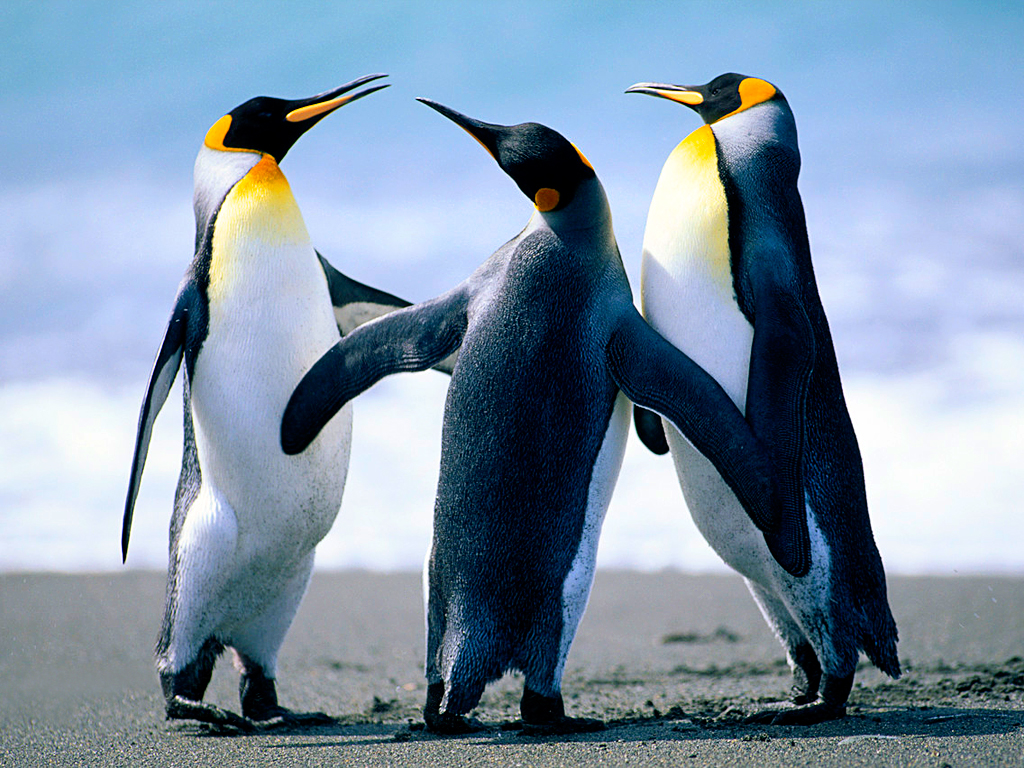
\includegraphics[scale=.50]{figures/Penguins.jpg}
\caption{TAMU figure - This is an example of a long figure title with a landscape figure.  Figure titles need to be single-spaced within and double spaced between in the list of figures.}
\label{fig:tamu-fig1-1}
\end{sidewaysfigure}
%%%%%%%%%%%%%%%%%%%%%%%%%%%%%%%%%%%%%%%%%%%%%%%%%%%%%%

More text here goes here.


Lorem ipsum dolor sit amet, consectetur adipiscing elit. Morbi augue urna, varius quis facilisis ac, imperdiet et nunc. Vestibulum ante ipsum primis in faucibus. 

\section{Testing the Top of the Page}
Maecenas accumsan lobortis dui fringilla suscipit. Quisque congue fringilla dui, sed eleifend sapien fringilla euismod. Pellentesque habitant morbi tristique senectus et netus et malesuada fames ac turpis egestas. Maecenas venenatis posuere magna quis tempus. Cras at leo massa, eu ultricies tellus. Nunc nec dictum augue. Cum sociis natoque penatibus et magnis dis parturient montes, nascetur ridiculus mus. Phasellus purus felis, mollis id scelerisque in, viverra in elit. Nulla iaculis ultrices justo, ac pharetra nisl rhoncus pulvinar. Duis vitae mauris velit, in congue massa.

Donec lectus orci, bibendum ut blandit dignissim, molestie non eros. Praesent aliquet feugiat dignissim. Morbi porttitor sollicitudin nisl, non mollis quam ultrices sit amet. Cras feugiat lacinia diam ut convallis. Nam nec varius ante. Nunc a ultrices felis. Quisque luctus sapien et ligula ornare quis consequat urna aliquet. Vestibulum vulputate lorem a tellus auctor id commodo risus sodales. Suspendisse quis tortor a felis molestie laoreet ut a nunc. Donec gravida sapien eget mauris condimentum lacinia. Proin eu purus libero. Nullam augue mi, vestibulum in convallis eu, adipiscing ac arcu. Donec nisi libero, egestas et molestie in, mollis quis ipsum. Sed gravida quam sit amet ante tempus rutrum non in mi. Cras viverra facilisis eros, id vestibulum sapien malesuada eget. Maecenas imperdiet luctus nisi vitae suscipit.



Aliquam erat volutpat. Integer ut mauris elit. Nam et lectus vel neque vehicula commodo. Integer at risus ligula. Fusce mollis mauris sed lorem aliquam bibendum porttitor tellus blandit. Curabitur enim nibh, accumsan eu elementum id, rutrum a ipsum. Vivamus ultricies, elit id ornare iaculis, metus justo posuere quam, sit amet bibendum arcu dolor a eros. Sed in nisl nibh. Aenean egestas est ut tortor volutpat vehicula. Maecenas aliquet placerat nunc hendrerit dictum. In et nisi massa. Pellentesque luctus, sapien quis dignissim vulputate, sapien libero bibendum velit, vitae auctor ipsum nulla at augue. Nulla ac eros vitae tortor elementum vehicula.

Morbi tristique egestas placerat. Cras faucibus eleifend porta. Class aptent taciti sociosqu ad litora torquent per conubia nostra, per inceptos himenaeos. Ut a pellentesque neque. Donec sollicitudin metus varius nulla egestas laoreet. Duis non mauris ut nunc adipiscing volutpat. Nam vitae est sed turpis tristique varius. 

\subsection{This is a Very Long Subsection Title This is a Very Long Subsection Title}

More text
\subsection{Subsection}

Subsection text

\section{Another Section}

Section text

\chapter{METHODOLOGY}

%===============================================================================
\section{Model Equations}
%===============================================================================
\subsection{Conservation Law Systems}
  A general system of conservation law equations is
\begin{equation}
  \ppt{\vectorsolution} + \divergence\consfluxvector
  = \mathbf{0} \eqc
\end{equation}
where $\vectorsolution$ is a vector of conserved quantities and
$\consfluxvector$ is the vector of conservation law flux
functions. When a conservation law does not fit this model equation,
a source term must be added:
\begin{equation}
  \ppt{\vectorsolution} + \nabla\cdot\consfluxvector
  = \conssource \eqp
\end{equation}
Table \ref{tab:cons_law_systems} gives some examples of conservation law
systems.
\begin{mytable}{Conservation Law Systems}{cons_law_systems}{l c c c}
{\emph{System} & $\vectorsolution$ & $\consfluxvector$ & $\conssource$}
\\
Burgers equation & $\scalarsolution$ & $\half\scalarsolution^2$ & 0\\ [1ex]\\
Euler equations &
  $\left[\begin{array}{c}\density\\\momentum\\\totalenergy\end{array}\right]$ &
  $\left[\begin{array}{c}\momentum\\
    \momentum\otimes\velocity + \pressure\mathbb{I}\\
    \pr{\totalenergy + \pressure}\velocity\end{array}\right]$ &
  $\mathbf{0}$\\ [1ex]\\
Shallow water equations &
  $\left[\begin{array}{c}\height\\\heightmomentum\end{array}\right]$ &
  $\left[\begin{array}{c}\heightmomentum\\
    \heightmomentum\otimes\velocity + \half\gravity\height^2\mathbb{I}
    \end{array}\right]$ &
  $\left[\begin{array}{c}0\\-\gravity\height\nabla\bathymetry\end{array}
    \right]$\\ [1ex]\\
\end{mytable}


\subsection{Scalar Conservation Laws}
  The primary application of this research is radiation transport,
as given by Equation \eqref{eq:rad_transport};
however, most of the analysis performed is valid
for any scalar conservation law of the following form:
\begin{equation}\label{eq:scalar_transport}
   \ppt{\scalarsolution} + \divergence\consfluxscalar
   + \reactioncoef\xt \scalarsolution\xt = \scalarsource\xt \eqc
\end{equation}
where $\scalarsolution\xt$ is a general scalar conserved quantity at position
$\x$ and time $\timevalue$, $\consfluxscalar$ is a general flux
function,
$\reactioncoef \xt\geq 0$ is a reaction coefficient, and $\scalarsource\xt \geq 0$ is a source
term.
Note that traditional FCT methodology does not consider the
the presence of the reaction term $\reactioncoef\xt \scalarsolution\xt$
or source term $\scalarsource\xt$ \cite{kuzmin_FCT}; extension to include these
terms is a significant driver for this research since this allows the application
of FCT to radiation transport, for example.
Since the radiation transport equation has a linear flux function
$\consfluxscalar$, hereafter it is assumed that
$\consfluxscalar\equiv\velocity\scalarsolution$, where $\velocity$ is a constant
velocity.

The radiation transport equation given by Equation
\eqref{eq:rad_transport} fits the model of
Equation \eqref{eq:scalar_transport}
by making the following substitutions:
\[
  \scalarsolution\rightarrow\angularflux
  \eqc \quad
  \velocity\rightarrow\speed\directionvector
  \eqc \quad
  \reactioncoef\rightarrow\speed\totalcrosssection
  \eqc \quad
  \scalarsource\rightarrow\speed\radiationsource
  \eqc
\]

Initial conditions are included if the problem is transient:
\begin{equation}
   \scalarsolution(\x,0) = \scalarsolution^0(\x)
   \quad \forall \x\in\domain \eqp
\end{equation}
Boundary conditions will depend on the chosen conservation law and
the particular problem. 
This research assumes an incoming flux boundary condition, which is strongly
imposed as a Dirichlet boundary condition:
\begin{equation}\label{eq:incoming_flux}
   \scalarsolution\xt = \scalarsolution^{\text{inc}}\xt \quad \forall \x
   \in \domainboundary^-,
     \quad \domainboundary^- = \{\x\in\domainboundary:
     \velocity\cdot\normalvector(\x)<0\} \eqp
\end{equation}
These conditions together make the problem well-posed, but for general
nonlinear conservation laws, care must be taken to ensure that the
boundary conditions used result in a well-posed problem.

\subsection{The Burgers Equation}
%  \input{content/preliminaries/burgers}
\subsection{The Shallow Water Equations\label{sec:shallowwater}}
  The shallow water equations, also known as the Saint-Venant equations, are an
approximation of conservation of mass and momentum equations applied to free
surface flows, which assume the fluid to be incompressible, non-viscous, and
non-heat-conducting. The shallow water equations make the additional
approximation that the depth component of acceleration can be neglected due to
horizontal length scales being much greater than the depth length
scale. Depth-integrating the conservation equations gives the shallow
water equations\cite{toro2009}\cite{leveque2002}:
\begin{equation}
\begin{gathered}
  \ppt{\vectorsolution} + \nabla\cdot\consfluxvector(\vectorsolution)
  = \conssource(\vectorsolution) \eqc
\\
  \vectorsolution
    = \left[\begin{array}{c}
        \height\\
        \heightmomentumx\\
        \heightmomentumy
      \end{array}\right]
  \eqc\quad
  \consfluxvector(\vectorsolution)
  = \left[\begin{array}{c c}
      \heightmomentumx & \heightmomentumy\\
      \frac{\heightmomentumx^2}{\height} + \half\gravity\height^2
        & \frac{\heightmomentumx\heightmomentumy}{\height}\\
      \frac{\heightmomentumx\heightmomentumy}{\height}
        & \frac{\heightmomentumy^2}{\height} + \half\gravity\height^2\\
    \end{array}\right]
  \eqc\quad
  \conssource(\vectorsolution)
  = \left[\begin{array}{c}
      0\\
     -\gravity\height\pd{\bathymetry}{x}\\
     -\gravity\height\pd{\bathymetry}{y}\\
    \end{array}\right]
  \eqc
\end{gathered}
\end{equation}
written more concisely as
\[
  \vectorsolution
    = \left[\begin{array}{c}\height\\\heightmomentum\end{array}\right]
  \eqc\quad
  \consfluxvector(\vectorsolution)
  = \left[\begin{array}{c}\heightmomentum\\
      \frac{\heightmomentum\otimes\heightmomentum}{\height}
      + \half\gravity\height^2\identity
    \end{array}\right]
  \eqc\quad
  \conssource(\vectorsolution)
  = \left[\begin{array}{c}0\\-\gravity\height\nabla\bathymetry\end{array}
    \right] \eqc
\]
where $\height$ is the height of the water, which plays the role of density
in the continuity equation, $\heightmomentum=\height\velocity$ is sometimes
referred to as \emph{discharge} and plays the role of momentum (hereafter,
$\heightmomentum$ will usually just be referred to as ``momentum''),
$\velocity$ is velocity, $\gravity$
is acceleration due to gravity, and $\bathymetry$ is the topography of the
bottom terrain of the fluid body, hereafter referred to as the \emph{bathymetry}
function.

Note that the shallow water equations are only valid in 1-D or 2-D, not 3-D,
since they are depth-integrated equations.

To complete the problem formulation, boundary
conditions must be provided, some examples being
Dirichlet boundary conditions, open boundary conditions,
wall boundary conditions,
etc. One must be careful with specifying boundary conditions to have
a well-posed problem for hyperbolic systems; a characteristic analysis
is required and there is a large body of research
addressing this area alone. For simplicity, problems are
chosen such that initial data never reaches the boundary
or boundary conditions are implemented as natural conditions
rather than using the method of characteristics.

For transient problems, initial conditions are specified:
\begin{equation}
   \vectorsolution(\x,0) = \vectorsolution^0(\x)
   \quad \forall \x\in\domain \eqp
\end{equation}

\subsection{The Euler Equations}
%  \input{content/preliminaries/euler}
%===============================================================================
\section{Discretization}
%===============================================================================
\subsection{Spatial Discretization\label{sec:spatial_discretization}}
  The continuous Galerkin (CG) finite element method (FEM) is used for spatial
discretization.  The numerical solution is thus approximated using an
expansion of basis functions $\testfunction_j(\x)$:
\begin{equation}
  \approximatescalarsolution\xt = \sumj \solutionletter_j(\timevalue)
  \testfunction_j(\x) \eqc
\end{equation}
where the coefficients $\solutionletter_j(\timevalue)$ are the basis function
expansion coefficients at time $\timevalue$. Substituting the approximate
solution into Equation \eqref{eq:cons_law} and testing with basis function
$\testfunction_i(\x)$ gives
\begin{equation}
   \intSi\ppt{\approximatescalarsolution}\testfunction_i(\x) d\volume
      + \intSi\left(\divergence\consfluxscalar[\approximatescalarsolution]
      + \reactioncoef(\x)\approximatescalarsolution\xt\right)
      \testfunction_i(\x) d\volume
      = \intSi \scalarsource\xt \testfunction_i(\x) d\volume \eqc
\end{equation}
where $\support_i$ is the support of $\testfunction_i(\x)$. If the flux function
$\consfluxscalar$ is linear, then the system to be solved is linear:
\begin{equation}\label{eq:semidiscrete}
  \consistentmassmatrix\ddt{\solutionvector}+\ssmatrix\solutionvector(t)
  = \ssrhs(\timevalue) \eqc
\end{equation}
where $\ssmatrix$ is the steady-state system matrix and $\solutionvector$ is the
vector of discrete solution values. If the velocity field $\velocity$ is
constant, then the elements of $\ssmatrix$ are
\begin{equation}\label{eq:Aij}
  \ssmatrixletter\ij \equiv \intSij\left(
  \velocity\cdot\nabla\testfunction_j(\x) +
  \reactioncoef(\x)\testfunction_j(\x)\right)\testfunction_i(\x) d\volume \eqc
\end{equation}
where $\support\ij$ is the dual support of $\testfunction_i(\x)$ and
$\testfunction_j(\x)$.  Otherwise, the divergence of the velocity field
appears:
\begin{equation}\label{eq:Aij_nonconstant_v}
  \ssmatrixletter\ij \equiv \intSij\left(
  \velocity\cdot\nabla\testfunction_j(\x) +
  (\reactioncoef(\x)+\divergence\velocity)\testfunction_j(\x)\right)
  \testfunction_i(\x) d\volume \eqp
\end{equation}
If the flux function $\consfluxscalar$ is nonlinear, then the system is
nonlinear, but it may be expressed in a quasilinear form:
\begin{equation}\label{eq:semi_quasilinear}
   \consistentmassmatrix\ddt{\solutionvector}
   + \ssmatrix(\approximatescalarsolution)\solutionvector(\timevalue)
   = \ssrhs(\timevalue) \eqc
\end{equation}
where $\approximatescalarsolution\xt$ is the numerical solution, and the
quasilinear matrix (i.e., the Jacobian matrix) entries are
\begin{equation}\label{eq:Aij_nonlinear}
  \ssmatrixletter\ij(\approximatescalarsolution) \equiv \intSij\left(
  \mathbf{\consfluxletter}'(\approximatescalarsolution)\cdot\nabla
  \testfunction_j(\x) +
  (\reactioncoef(\x)+\nabla\cdot\velocity)\testfunction_j(\x)\right)
  \testfunction_i(\x) d\volume \eqp
\end{equation}
The elements of $\ssrhs(\timevalue)$ are
\begin{equation}
  \ssrhsletter_i(\timevalue) \equiv \intSi \scalarsource\xt\testfunction_i(\x)
  d\volume \eqp
\end{equation}
$\consistentmassmatrix$ is the consistent mass matrix, which has the entries
\begin{equation}\label{eq:massmatrix}
  \massmatrixletter^C\ij \equiv \intSij
  \testfunction_j(\x)\testfunction_i(\x) d\volume \eqp
\end{equation}
Similarly, for the linear steady-state case, the linear system is
\begin{equation}
  \ssmatrix\solutionvector = \ssrhs \eqc
\end{equation}
or for the nonlinear case,
\begin{equation}
  \ssmatrix(\approximatescalarsolution)\solutionvector = \ssrhs \eqp
\end{equation}

  \subsubsection{The Shallow Water Equations}
  The shallow water equations, also known as the Saint-Venant equations, are an
approximation of conservation of mass and momentum equations applied to free
surface flows, which assume the fluid to be incompressible, non-viscous, and
non-heat-conducting. The shallow water equations make the additional
approximation that the depth component of acceleration can be neglected due to
horizontal length scales being much greater than the depth length
scale. Depth-integrating the conservation equations gives the shallow
water equations\cite{toro2009}\cite{leveque2002}:
\begin{equation}
\begin{gathered}
  \ppt{\vectorsolution} + \nabla\cdot\consfluxvector(\vectorsolution)
  = \conssource(\vectorsolution) \eqc
\\
  \vectorsolution
    = \left[\begin{array}{c}
        \height\\
        \heightmomentumx\\
        \heightmomentumy
      \end{array}\right]
  \eqc\quad
  \consfluxvector(\vectorsolution)
  = \left[\begin{array}{c c}
      \heightmomentumx & \heightmomentumy\\
      \frac{\heightmomentumx^2}{\height} + \half\gravity\height^2
        & \frac{\heightmomentumx\heightmomentumy}{\height}\\
      \frac{\heightmomentumx\heightmomentumy}{\height}
        & \frac{\heightmomentumy^2}{\height} + \half\gravity\height^2\\
    \end{array}\right]
  \eqc\quad
  \conssource(\vectorsolution)
  = \left[\begin{array}{c}
      0\\
     -\gravity\height\pd{\bathymetry}{x}\\
     -\gravity\height\pd{\bathymetry}{y}\\
    \end{array}\right]
  \eqc
\end{gathered}
\end{equation}
written more concisely as
\[
  \vectorsolution
    = \left[\begin{array}{c}\height\\\heightmomentum\end{array}\right]
  \eqc\quad
  \consfluxvector(\vectorsolution)
  = \left[\begin{array}{c}\heightmomentum\\
      \frac{\heightmomentum\otimes\heightmomentum}{\height}
      + \half\gravity\height^2\identity
    \end{array}\right]
  \eqc\quad
  \conssource(\vectorsolution)
  = \left[\begin{array}{c}0\\-\gravity\height\nabla\bathymetry\end{array}
    \right] \eqc
\]
where $\height$ is the height of the water, which plays the role of density
in the continuity equation, $\heightmomentum=\height\velocity$ is sometimes
referred to as \emph{discharge} and plays the role of momentum (hereafter,
$\heightmomentum$ will usually just be referred to as ``momentum''),
$\velocity$ is velocity, $\gravity$
is acceleration due to gravity, and $\bathymetry$ is the topography of the
bottom terrain of the fluid body, hereafter referred to as the \emph{bathymetry}
function.

Note that the shallow water equations are only valid in 1-D or 2-D, not 3-D,
since they are depth-integrated equations.

To complete the problem formulation, boundary
conditions must be provided, some examples being
Dirichlet boundary conditions, open boundary conditions,
wall boundary conditions,
etc. One must be careful with specifying boundary conditions to have
a well-posed problem for hyperbolic systems; a characteristic analysis
is required and there is a large body of research
addressing this area alone. For simplicity, problems are
chosen such that initial data never reaches the boundary
or boundary conditions are implemented as natural conditions
rather than using the method of characteristics.

For transient problems, initial conditions are specified:
\begin{equation}
   \vectorsolution(\x,0) = \vectorsolution^0(\x)
   \quad \forall \x\in\domain \eqp
\end{equation}

\subsection{Temporal Discretization\label{sec:temporal_discretization}}
  \subsubsection{Explicit Euler Scheme}
    Considering a time step from time $\timevalue^\timeindex$ to time
$\timevalue^{\timeindex+1}$ with time step size $\timestepsize\equiv
\timevalue^{\timeindex+1}-\timevalue^\timeindex$, the semi-discrete equation
given by Equation \eqref{eq:semidiscrete} is discretized using the explicit
Euler:
\begin{equation}\label{eq:galerkin_FE}
   \consistentmassmatrix\frac{\solutionvector^{\timeindex+1}
   -\solutionvector^\timeindex}{\timestepsize}
   +\ssmatrix\solutionvector^\timeindex = \ssrhs^\timeindex,
\end{equation}
where $\solutionvector^{\timeindex+1}$ is the Galerkin solution at time
$\timevalue^{\timeindex+1}$.

  \subsubsection{Strong Stability-Preserving Runge-Kutta (SSPRK)
    Schemes\label{sec:ssprk}}
    Strong Stability-Preserving Runge Kutta (SSPRK) methods are a class of multistage
Runge Kutta methods that offer high-order accuracy while preserving stability.
The subset of SSPRK methods considered in this research conform to the
following form for a given time step $\timevalue^\timeindex\rightarrow
\timevalue^{\timeindex+1}$,
where $\RKstagesolution^i$ denotes the $i$th stage solution:
\begin{equation}
  \RKstagesolution^i = \RKoldsolutioncoef_i\RKstagesolution^0
  + \RKstagesolutioncoef_i\RKintermediatesolution^i \eqc
\end{equation}
where $\timestepsize=\timevalue^{\timeindex+1}-\timevalue^\timeindex$,
$\RKstagesolution^0=\solutionvector^\timeindex$, and
$\RKintermediatesolution^i$ is the solution of the following forward Euler
step:
\begin{equation}
   \massmatrix\RKintermediatesolution^i = \massmatrix\RKstagesolution^{i-1}
   + \timestepsize(\ssrhs(\RKstagetime_i)
   - \ssmatrix(\RKstagetime_i)\RKstagesolution^{i-1}) \eqc
\end{equation}
where $\RKstagetime_i = \timevalue^\timeindex+\RKtimecoef_i\timestepsize$,
$\massmatrix$ is the mass matrix, $\ssrhs(\timevalue)$ is the steady-state
right hand side vector, and $\ssmatrix(\timevalue)$ is the steady-state matrix.
Therefore the function performs a time step that is similar to an explicit
Euler step, except that the steady-state residual is not necessarily evaluated
at time $\timevalue^\timeindex$. The new solution
$\solutionvector^{\timeindex+1}$ is the final stage solution:
\begin{equation}
   \solutionvector^{\timeindex+1} = \RKstagesolution^\RKnstages \eqc
\end{equation}
where $\RKnstages$ is the number of stages for the scheme.

The Explicit Euler scheme can be expressed as a 1-stage SSPRK method with
with the following coefficients:
\begin{equation}
   \RKoldsolutioncoef_1 = 0\qquad\RKstagesolutioncoef_1 = 1\qquad \RKtimecoef_1
   = 0 \eqc
\end{equation}
and the 3-stage, 3rd-order accurate SSPRK scheme (also known as the Shu-Osher
scheme), has the following coefficients:
\begin{equation}
  \RKoldsolutioncoef = \left[\begin{array}{c}
    0\\\frac{3}{4}\\\frac{1}{3}\end{array}\right]
  \qquad\RKstagesolutioncoef = \left[\begin{array}{c}
    1\\\frac{1}{4}\\\frac{2}{3}\end{array}\right]
  \qquad c = \left[\begin{array}{c}0\\1\\\frac{1}{2}\end{array}\right] \eqp
\end{equation}

  \subsubsection{Theta Schemes\label{sec:theta}}
    Discretizing Equation \eqref{eq:semidiscrete} with the $\theta$ scheme gives
\begin{equation}\label{eq:galerkin_theta}
  \consistentmassmatrix\frac{\solutionvector^{\timeindex+1}
  - \solutionvector^\timeindex}{\timestepsize}
  + (1-\theta)\ssmatrix\solutionvector^\timeindex
  + \theta\ssmatrix\solutionvector^{\timeindex+1}
  = (1-\theta)\ssrhs^\timeindex + \theta\ssrhs^{\timeindex+1}.
\end{equation}
Note that $\theta=0$ corresponds to the explicit Euler method,
$\theta=1$ corresponds to the implicit Euler method, and $\theta=\half$
corresponds to the Crank-Nicolson method.

%===============================================================================
\section{Low-Order Schemes}  
%===============================================================================
\subsection{Low-Order Viscosity\label{sec:low_order_viscosity}}
  In this section, a graph-theoretic approach is taken to define a low-order
scheme that is monotone and maximum principle preserving. The following
bilinear form is employed in the low-order scheme:
%--------------------------------------------------------------------------------
\begin{definition}{Local Viscous Bilinear Form}
   The local viscous bilinear form for cell $\cell$ is defined as follows:
   \begin{equation}\label{eq:bilinearform}
     \localviscbilinearform{\cell}{j}{i} \equiv \left\{\begin{array}{l l}
       -\frac{1}{\cardinality - 1}\cellvolume & i\ne j
       \quad i,j\in \indicescell \\
       \cellvolume & i = j \eqc \quad i,j\in \indicescell \\
       0           & i\notin\indicescell \quad | \quad j\notin\indicescell
     \end{array}\right. \eqc
   \end{equation}
   with $\indicescell$ being the set of indices corresponding to degrees of
   freedom in the support of cell $\cell$:
   \begin{equation}
     \indicescell \equiv \{j\in\{1,\ldots,N\}: |\support_j\cap \celldomain|\ne 0\}
     \eqc
   \end{equation}
   $\cardinality$ being the number of elements in the set $\indicescell$,
   i.e., the set's cardinality:
   \begin{equation}
     \cardinality \equiv \textup{card}(\indicescell) \eqc
   \end{equation} 
   and $\cellvolume$ being the cell volume.
\end{definition}
%--------------------------------------------------------------------------------
The definition of the low-order viscosity follows.
%--------------------------------------------------------------------------------
\begin{definition}{Low-Order Viscosity}
   The low-order viscosity for cell $\cell$ is defined as follows:
   \begin{equation}
     \lowordercellviscosity[\timeindex] \equiv \max\limits_{i\ne j\in\indicescell}
     \frac{\max(0,\ssmatrixletter\ij^\timeindex)}
     {-\mkern-20mu\sumKSij[T]\mkern-20mu\localviscbilinearform{T}{j}{i}}
     \eqc
   \end{equation}
   where $\ssmatrixletter\ij^\timeindex$ is the $i,j$th entry of the Galerkin
   steady-state matrix given by Equation \eqref{eq:Aij}, and
   $\support\ij=\support_i\cap \support_j$ is the dual-support of test
   functions $\testfunction_i$ and $\testfunction_j$.
\end{definition}
%--------------------------------------------------------------------------------

\subsection{The Low-Order System\label{sec:low_order_system}}
  The low-order system uses a steady-state system matrix that is augmented
to include the low-order diffusion matrix. Definitions of the low-order
diffusion matrix and low-order system matrix follow.
%--------------------------------------------------------------------------------
\begin{definition}{Low-Order Artificial Diffusion Matrix}
   The low-order artificial diffusion matrix $\loworderdiffusionmatrix[\timeindex]$
   is assembled using the low-order viscosity and local viscous bilinear
   form introduced in Section \ref{sec:low_order_viscosity}:
   \begin{equation}\label{eq:low_order_diffusion_matrix}
     \diffusionmatrixletter\ij^{L,\timeindex} \equiv
       \sumKSij\mkern-20mu\lowordercellviscosity[\timeindex]
       \localviscbilinearform{\cell}{j}{i} \eqp
   \end{equation}
\end{definition}
%--------------------------------------------------------------------------------
\begin{definition}{Low-Order Steady-State System Matrix}
   The low-order steady-state system matrix is the sum of the inviscid 
   steady-state system matrix $\ssmatrix[\timeindex]$ and the low-order diffusion
   matrix $\loworderdiffusionmatrix[\timeindex]$:
   \begin{equation}\label{eq:low_order_ss_matrix}
      \loworderssmatrix[\timeindex] \equiv
        \ssmatrix[\timeindex] + \loworderdiffusionmatrix[\timeindex] \eqp
   \end{equation}
\end{definition}
%--------------------------------------------------------------------------------
For the low-order system, the mass matrix is lumped, i.e.,
$\consistentmassmatrix\rightarrow\lumpedmassmatrix$, where
\begin{equation}
  \massmatrixletter^L_{i,j} = \left\{\begin{array}{l l}
    \sum\limits_k \massmatrixletter^C_{i,k} & j = i\\
    0                                       & \mbox{otherwise}
    \end{array}\right.
    \eqc
\end{equation}
and the low-order
steady-state system matrix defined in Equation \eqref{eq:low_order_ss_matrix}
is used. The low-order system for different time discretizations follows:
\begin{center}{\textbf{Steady-state scheme}:}\end{center}
\begin{equation}\label{eq:low_ss}
   \loworderssmatrix\lowordersolution = \ssrhs
\end{equation}
\begin{center}{\textbf{Semidiscrete scheme}:}\end{center}
\begin{equation}\label{eq:low_semidiscrete}
   \lumpedmassmatrix\ddt{\lowordersolution}
    + \loworderssmatrix(\timevalue)\lowordersolution(\timevalue) 
    = \ssrhs(\timevalue)
\end{equation}
\begin{center}{\textbf{Explicit Euler scheme}:}\end{center}
\begin{equation}\label{eq:low_explicit_euler}
  \lumpedmassmatrix\frac{\lowordersolution-\solutionvector^{\timeindex}}
  {\timestepsize}
  + \loworderssmatrix[\timeindex]\solutionvector^{\timeindex}
  = \ssrhs^\timeindex
\end{equation}
\begin{center}{\textbf{Theta scheme}:}\end{center}
\begin{equation}\label{eq:low_theta}
  \lumpedmassmatrix\frac{\lowordersolution-\solutionvector^\timeindex}
  {\timestepsize}
  + (1-\theta)\loworderssmatrix[\timeindex]\solutionvector^\timeindex
  + \theta\loworderssmatrix[\timeindex+1]\lowordersolution
  = (1-\theta)\ssrhs^\timeindex + \theta\ssrhs^{\timeindex+1}
\end{equation}

\subsection{M-Matrix Property}
  In this section, it will be shown that the low-order steady-state system matrix
defined in Equation \eqref{eq:low_order_ss_matrix} is an M-matrix, which allows
a discrete maximum principle for the low-order solution to be proven in Section
\ref{sec:DMP}.
%--------------------------------------------------------------------------------
\begin{lemma}[lem:offdiagonalnegative]{Non-Positivity of Off-Diagonal Elements}
   The off-diagonal elements of the linear system matrix are non-positive:
   \[
     \ssmatrixletter^{L,\timeindex}\ij\le 0, \quad j\ne i \eqp
   \]
\end{lemma}

\begin{proof}
This proof begins by bounding the term $\diffusionmatrixletter\ij^{L,\timeindex}$:
\begin{eqnarray*}
   \diffusionmatrixletter\ij^{L,\timeindex}=
     \sumKSij\mkern-20mu\lowordercellviscosity[\timeindex]
   \localviscbilinearform{\cell}{j}{i}
   & = & \sumKSij\max\limits_{k\ne \ell\in \indicescell}
     \pr{\frac{\max(0,\ssmatrixletter_{k,\ell}^\timeindex)}
       {\mkern10mu-\mkern-20mu\sum\limits_{T:\celldomain[T]\subset\support_{k,\ell}}
       \mkern-20mu\localviscbilinearform{T}{\ell}{k}}}
     \localviscbilinearform{\cell}{j}{i} \eqp
\end{eqnarray*}
Since $\localviscbilinearform{\cell}{j}{i} < 0$ for $j\ne i$ and $y_i \leq
\max_j y_j$,
\begin{eqnarray*}
   \diffusionmatrixletter\ij^{L,\timeindex} & \le &
     \sumKSij \frac{\max(0,\ssmatrixletter\ij^\timeindex)}
   {\mkern10mu-\mkern-20mu\sumKSij[T]\mkern-20mu\localviscbilinearform{T}{j}{i}}
   \localviscbilinearform{\cell}{j}{i} \eqc\\
   &  =  & -\max(0,\ssmatrixletter\ij^\timeindex)
     \frac{\sumKSij\mkern-20mu\localviscbilinearform{\cell}{j}{i}}
     {\sumKSij[T]\mkern-20mu\localviscbilinearform{T}{j}{i}} \eqc\\
   &  =  & -\max(0,\ssmatrixletter\ij^\timeindex) \eqc\\
   & \le & -\ssmatrixletter\ij^\timeindex \eqp
\end{eqnarray*}
Applying this inequality to Equation \eqref{eq:low_order_ss_matrix} gives
\begin{eqnarray*}
  \ssmatrixletter^{L,\timeindex}\ij &  =  &
    \ssmatrixletter\ij^\timeindex + \diffusionmatrixletter\ij^{L,\timeindex}
    \eqc\\
  \ssmatrixletter^{L,\timeindex}\ij & \le &
    \ssmatrixletter\ij^\timeindex - \ssmatrixletter\ij^\timeindex
    \eqc\\
  \ssmatrixletter^{L,\timeindex}\ij & \le & 0 \eqp \qed
\end{eqnarray*}
\end{proof}
%--------------------------------------------------------------------------------
\begin{lemma}[lem:diagonalpositive]{Non-Negativity of Diagonal Elements}
   The diagonal elements  of the linear system matrix are non-negative:
   \[
     \ssmatrixletter^{L,\timeindex}_{i,i}\ge 0 \eqp
   \]
\end{lemma}

\begin{proof}
The diagonal elements of the low-order system matrix are
\[
  \ssmatrixletter^{L,\timeindex}_{i,i} =
    \intSi\mathbf{\consfluxletter}'(\approximatescalarsolution^\timeindex)\cdot
    \nabla\testfunction_i(\x)\testfunction_i(\x)d\volume
  + \intSi\sigma(\x)\testfunction_i^2(\x)d\volume
  + \sumKSi\mkern-15mu\lowordercellviscosity[\timeindex]
    \localviscbilinearform{\cell}{i}{i}
  \eqp
\]
To prove that $\ssmatrixletter^{L,\timeindex}_{i,i}$ is non-negative, it is sufficient to
prove that each term in the above expression is non-negative. The
non-negativity of the interaction term and viscous term are obvious
($\reactioncoef \ge 0, \, \lowordercellviscosity[\timeindex]\ge 0, \,
\localviscbilinearform{\cell}{i}{i}>0$), but the non-negativity of the divergence
term is not necessarily obvious. On the interior of the domain, the divergence
term gives zero contribution because the divergence integral may be transformed
into a surface integral
$\intSi\mathbf{\consfluxletter}'(\approximatescalarsolution^\timeindex)
\cdot\normalvector\frac{\testfunction_i^2}{2} d\area$ via the
divergence theorem; one can then recognize that the basis function
$\testfunction_i$ evaluates to zero on the boundary of its support
$\support_i$. On the outflow boundary of the domain, the term
$\mathbf{\consfluxletter}'(\approximatescalarsolution^\timeindex)
\cdot\normalvector \frac{\testfunction_i^2}{2}$ is positive because
$\mathbf{\consfluxletter}'(\approximatescalarsolution^\timeindex)
\cdot\normalvector > 0$ for an outflow boundary. This quantity is of
course negative for the inflow boundary, so one must consider the boundary
conditions applied for incoming boundary nodes to determine if this condition
is true and a discrete maximum principle applies. For instance, if a Dirichlet boundary condition is
applied, then a discrete maximum principle does not apply.
strongly imposed on the incoming boundary, so for degrees of freedom $i$ on the
incoming boundary, $\ssmatrixletter^{L,\timeindex}_{i,i}$ will be set equal to some positive
value such as 1 with a corresponding incoming value accounted for in the right
hand side $\ssrhs$ of the linear system.\qed
\end{proof}
%--------------------------------------------------------------------------------
\begin{lemma}{Non-Negativity of Row Sums}
   The sum of all elements in a row $i$ is non-negative:
   \[
     \sumj \ssmatrixletter^{L,\timeindex}\ij \ge 0 \eqp
   \]
\end{lemma}

\begin{proof}
Using the fact that $\sumj\testfunction_j(\x)=1$ and
$\sumj \localviscbilinearform{\cell}{j}{i}=0$,
\begin{eqnarray*}
   \sumj \ssmatrixletter^{L,\timeindex}\ij & = & \sumj \intSij
      \left(\mathbf{\consfluxletter}'(\approximatescalarsolution^\timeindex)
        \cdot\nabla\testfunction_j(\x) +
      \reactioncoef(\x)\testfunction_j(\x)\right)\testfunction_i(\x) d\volume +
      \sumj\sumKSij\mkern-20mu\lowordercellviscosity[\timeindex]\localviscbilinearform{\cell}{j}{i}
      \eqc\\
   & = & \intSi\left(
      \mathbf{\consfluxletter}'(\approximatescalarsolution^\timeindex)\cdot
      \nabla\sumj\testfunction_j(\x) +
      \reactioncoef(\x)\sumj\testfunction_j(\x)\right)
      \testfunction_i(\x) d\volume \eqc\\
   \label{eq:rowsum} & = & \intSi\reactioncoef(\x)\testfunction_i(\x) d\volume
     \eqc\\
   &\ge& 0 \eqp \qed
\end{eqnarray*}
\end{proof}
%--------------------------------------------------------------------------------
\begin{lemma}[lem:diagonallydominant]{Diagonal Dominance}
   $\loworderssmatrix[\timeindex]$ is strictly diagonally dominant:
   \[
     \left|\ssmatrixletter^{L,\timeindex}_{i,i}\right|
     \ge \sumjnoti \left|\ssmatrixletter^{L,\timeindex}\ij\right| \eqp
   \]
\end{lemma}
\begin{proof}
Using the inequalities $\sumj \ssmatrixletter^{L,\timeindex}\ij \ge 0$ and
$\ssmatrixletter^{L,\timeindex}\ij\le 0, j\ne i$, it is proven that
$\loworderssmatrix[\timeindex]$ is strictly diagonally dominant:
\begin{eqnarray*}
  \sumj     \ssmatrixletter^{L,\timeindex}\ij       & \ge & 0 \eqc\\
  \sumjnoti \ssmatrixletter^{L,\timeindex}\ij
    + \ssmatrixletter^{L,\timeindex}_{i,i} & \ge & 0 \eqc\\
  \left|\ssmatrixletter^{L,\timeindex}_{i,i}\right| & \ge &
    \sumjnoti -\ssmatrixletter^{L,\timeindex}\ij
    \eqc\\
  \left|\ssmatrixletter^{L,\timeindex}_{i,i}\right| & \ge
    & \sumjnoti \left|\ssmatrixletter^{L,\timeindex}\ij\right| \eqp \qed
\end{eqnarray*}
\end{proof}
%--------------------------------------------------------------------------------
\begin{lemma}{M-Matrix}
  $\loworderssmatrix[\timeindex]$ is an M-Matrix.
\end{lemma}
\begin{proof}
To prove that a matrix is an M-Matrix, it is sufficient to prove that
the following 3 statements are true:
\begin{enumerate}
\item $\ssmatrixletter^{L,\timeindex}\ij\le 0, j\ne i$,
\item $\ssmatrixletter^{L,\timeindex}_{i,i}\ge 0$,
\item $\left|\ssmatrixletter^{L,\timeindex}_{i,i}\right|
      \ge \sumjnoti \left|\ssmatrixletter^{L,\timeindex}\ij\right|$.
\end{enumerate}
These conditions are proven by Lemmas \ref{lem:offdiagonalnegative},
\ref{lem:diagonalpositive}, and \ref{lem:diagonallydominant}, respectively.\qed
\end{proof}
%--------------------------------------------------------------------------------

\subsection{Discrete Maximum Principles\label{sec:DMP}}
  \begin{theorem}{Steady-State Scheme Local Discrete Maximum Principle}
The solution of the steady-state low-order system given
by Equation \eqref{eq:low_ss}
satisfies the following
local discrete maximum principle:
\begin{subequations}\label{eq:DMP_ss}
\begin{equation}
   \DMPlowerbound_i(\solutionvector^L)
     \leq \solutionletter_i^L
     \leq \DMPupperbound_i(\solutionvector^L)
     \quad\forall i \eqc
\end{equation}
\begin{equation}
   \DMPbounds_i(\solutionvector^L)
     \equiv -\frac{1}{\ssmatrixletter^L_{i,i}}
      \sumjnoti\ssmatrixletter^L_{i,j}
      \solutionletter_{\substack{\max\\\min},j\ne i}^L
      + \frac{\ssrhsletter_i}{\ssmatrixletter^L_{i,i}} \eqc
\end{equation}
\end{subequations}
where
\[
  \solutionletter_{\min,j\ne i}^L \equiv \min\limits_{j\ne i\in\indicescell[\support_i]}
    \solutionletter_j^L
  \eqc\quad
  \solutionletter_{\max,j\ne i}^L \equiv \max\limits_{j\ne i\in\indicescell[\support_i]}
    \solutionletter_j^L
  \eqp
\]
\end{theorem}

\begin{proof}
\begin{eqnarray*}
  \sumj\ssmatrixletter^L_{i,j}\solutionletter_j^L & = & \ssrhsletter_i\eqc\\
  \ssmatrixletter^L_{i,i}\solutionletter_i^L      & = & \sum\limits_{j\ne i}
    - \ssmatrixletter^L_{i,j}\solutionletter_j^L + \ssrhsletter_i\eqc\\
  \ssmatrixletter^L_{i,i}\solutionletter_i^L      & \le &
    \pr{\sumjnoti -\ssmatrixletter^L_{i,j}}\solutionletter_{\max,j\ne i}^L
    + \ssrhsletter_i\eqc\\
  \solutionletter_i^L & \le & -\frac{1}{\ssmatrixletter^L_{i,i}}
    \sumjnoti\ssmatrixletter^L_{i,j}\solutionletter_{\max,j\ne i}^L
    + \frac{\ssrhsletter_i}{\ssmatrixletter^L_{i,i}} \eqp
\end{eqnarray*}
A similar analysis is performed to prove the lower bound for
$\solutionletter_i^L$.\qed
\end{proof}

  %--------------------------------------------------------------------------------
\subsubsection{Explicit Euler}
%--------------------------------------------------------------------------------
\begin{theorem}{Explicit Euler Scheme Discrete Maximum Principle}{exloworderDMP}
If the CFL-like condition
\begin{equation}\label{ex_CFL}
   \Delta t \leq \frac{m_i}{A_{i,i}^L}\quad\forall i
   \qquad\Longleftrightarrow\qquad
   1 - \frac{\Delta t}{m_i}A_{i,i}^L \geq 0\quad\forall i,
\end{equation}
is satisfied, then the low-order solution obtained using the Explicit Euler
method satisfies the following discrete maximum principle:
\begin{equation}\label{explicit_max_principle}
   W_i^-\leq U_i^{L,n+1}\leq W_i^+\quad\forall i,
\end{equation}
where
\begin{equation}\label{ex_bounds}
   W_i^\pm\equiv U_{\substack{\max\\\min},i}^n\left(1-\frac{\Delta t}{m_i}
      \sum\limits_j A^L_{i,j}\right)
      + \frac{\Delta t}{m_i}b_i^n,
\end{equation}
where $U_{\substack{\max\\\min},i}^n =
\substack{\max\\\min\limits_{j\in \mathcal{I}(S_i)}}U_j^n$,
and $\mathcal{I}(S_i)$ is the set of indices of degrees of freedom in the
support of degree of freedom $i$.
\end{theorem}

\begin{proof}
Evaluating row $i$ of Equation \eqref{semidiscretelow} with Explicit Euler
and rearranging,
\[
   U_i^{L,n+1} = U_i^n - \frac{\Delta t}{m_i}\sum\limits_j U_j^n A^L_{i,j}
      + \frac{\Delta t}{m_i}b_i^n,
\]
where $m_i$ is the $i$th element of the lumped mass matrix.
Rearranging this equation,
\[
   U_i^{L,n+1} = \left(1-\frac{\Delta t}{m_i}A^L_{i,i}\right)U_i^n - \frac{\Delta t}{m_i}
      \sum\limits_{j\ne i} U_j^n A^L_{i,j} + \frac{\Delta t}{m_i}b_i^n,
\]
The CFL-like condition in Equation \eqref{ex_CFL} gives that $1-\frac{\Delta t}{m_i}A^L_{i,i} \ge 0$, and by
Lemma \ref{offdiagonalnegative}, it is known that the off-diagonal
elements $A^L_{i,j}, j\ne i$, are non-positive. Thus, the following inequality is
able to be applied:
\[
   U_i^{L,n+1} \le
   U_{\max,i}^n\left(1-\frac{\Delta t}{m_i}\sum\limits_j A^L_{i,j}\right)
      + \frac{\Delta t}{m_i}b_i^n,
\]
and similarly for the lower bound.\qed
\end{proof}

  %--------------------------------------------------------------------------------
\subsubsection{Theta Scheme}
%--------------------------------------------------------------------------------
\begin{theorem}{$\theta$-Scheme Discrete Maximum Principle}
If the CFL-like condition
\begin{equation}\label{theta_CFL}
   \Delta t \leq \frac{m_i}{(1-\theta)A_{i,i}^L}\quad\forall i
   \qquad\Longleftrightarrow\qquad
   1 - \frac{(1-\theta)\Delta t}{m_i}A_{i,i}^L \geq 0\quad\forall i
\end{equation}
is satisfied, then the low-order solution  obtained using the $\theta$-scheme
satisfies the following discrete maximum principle:
\begin{equation}\label{theta_max_principle}
   W_i^-\leq U_i^{L,n+1}\leq W_i^+\quad\forall i,
\end{equation}
where
\begin{equation}\label{theta_W}
   W_i^\pm \equiv \frac{1}{1+\frac{\theta\Delta t}{m_i}A_{i,i}^L}
     \left[\left(1 - \frac{(1-\theta)
     \Delta t}{m_i}\sum\limits_j A_{i,j}^L\right)U_{\substack{\max\\\min},i}^n
    -\frac{\theta\Delta t}{m_i}\sum\limits_{j\ne i}A_{i,j}^L
     U_{\substack{\max\\\min},i}^{L,n+1}
    +\frac{\Delta t}{m_i}\left((1-\theta)b_i^n + \theta b_i^{n+1}\right)\right],
\end{equation}
where $U_{\substack{\max\\\min},i}^n = \substack{\max\\\min\limits_{j\in
\mathcal{I}(S_i)}}U_j^n$,
$U_{\substack{\max\\\min},i}^{L,n+1} = \substack{\max\\\min\limits_{j\in
\mathcal{I}(S_i)}}U_j^{L,n+1}$,
and $\mathcal{I}(S_i)$ is the set of indices of degrees of freedom in the
support of degree of freedom $i$.
\end{theorem}
\begin{proof}
Evaluating row $i$ of Equation \eqref{semidiscretelow} with the $\theta$-scheme,
\[
  m_i\frac{U_i^{L,n+1}-U_i^n}{\Delta t}+\sum\limits_j A_{i,j}^L \left((1-\theta) U_j^n
  + \theta U_j^{L,n+1}\right) = (1-\theta)b_i^n + \theta b_i^{n+1},
\]
and rearranging,
\[
   U_i^{L,n+1} = \frac{1}{1+\frac{\theta\Delta t}{m_i}A_{i,i}^L}
     \left[\left(1 - \frac{(1-\theta)\Delta t}{m_i}A_{i,i}^L\right)U_i^n
    -\frac{\Delta t}{m_i}\sum\limits_{j\ne i}A_{i,j}^L
     \left(\theta U_j^{L,n+1}
    +(1-\theta) U_j^n\right)
    +\frac{\Delta t}{m_i}\left((1-\theta)b_i^n + \theta b_i^{n+1}\right)\right].
\]
By Lemma \ref{offdiagonalnegative}, it is known that the off-diagonal
elements $A^L_{i,j}, j\ne i$, are non-positive, and by Equation \ref{theta_CFL}
the term $1 - \frac{(1-\theta)\Delta t}{m_i}A_{i,i}^L$ is non-negative.
Thus, the following inequality is able to be applied:
\[
   U_i^L \le
     \frac{1}{1+\frac{\theta\Delta t}{m_i}A_{i,i}^L}
     \left[\left(1 - \frac{(1-\theta)
     \Delta t}{m_i}\sum\limits_j A_{i,j}^L\right)U_{\max,i}^n
    -\frac{\theta\Delta t}{m_i}\sum\limits_{j\ne i}A_{i,j}^L
     U_{\max,i}^{L,n+1}
    +\frac{\Delta t}{m_i}\left((1-\theta)b_i^n + \theta b_i^{n+1}\right)\right],
\]
and similarly for the lower bound.\qed
\end{proof}

%===============================================================================
\section{High-Order Schemes}  
%===============================================================================
\subsection{Entropy Viscosity\label{sec:entropy_viscosity}}
  \subsubsection{Entropy Viscosity for Scalar Conservation Law Equations
    \label{sec:entropy_viscosity_scalar}}
    To construct a high-order scheme, the concept of entropy viscosity is used in
conjunction with the bilinear form introduced in Equation
\eqref{eq:bilinearform}.  The high-order viscosity
$\highordercellviscosity[\timeindex]$ is computed as the minimum of the
low-order viscosity $\lowordercellviscosity$ and the entropy viscosity
$\entropycellviscosity[\timeindex]$:
\begin{equation}\label{eq:high_order_viscosity}
   \highordercellviscosity[\timeindex] = \min(\lowordercellviscosity,
   \entropycellviscosity[\timeindex]) \eqc
\end{equation}
where the entropy viscosity is defined as
\begin{equation}
   \entropycellviscosity[n] = \frac{\entropyresidualcoef
   \entropyresidual_\cellindex^\timeindex
   + \entropyjumpcoef\entropyjump_\cell^\timeindex}
   {\|\entropy(\approximatescalarsolution^\timeindex)
   -\bar{\entropy}(\approximatescalarsolution^\timeindex)\|_{L^\infty(\domain)}}
   \eqp
\end{equation}
The entropy is defined to be some convex function of $\scalarsolution$ such as
$\entropy(\scalarsolution)=\frac{1}{2}\scalarsolution^2$. The entropy residual
$\entropyresidual_\cellindex^\timeindex$ is the following:
\begin{equation}
  \entropyresidual_\cellindex^\timeindex
  \equiv \left\|\entropyresidual(\approximatescalarsolution^\timeindex,
  \approximatescalarsolution^{\timeindex-1})
  \right\|_{L^\infty(\cellindex)} \eqc
\end{equation}
\begin{equation}
  \entropyresidual(\approximatescalarsolution^\timeindex,
  \approximatescalarsolution^{\timeindex-1})
  \equiv \frac{\entropy(\approximatescalarsolution^\timeindex)
  - \entropy(\approximatescalarsolution^{\timeindex-1})} 
  {\timestepsize^\timeindex}
  + \entropy'(\approximatescalarsolution^\timeindex)\pr{
  \divergence\consfluxscalar[\approximatescalarsolution^\timeindex]
  + \reactioncoef \approximatescalarsolution^\timeindex
  - \scalarsource} \eqc
\end{equation}
where the $L^\infty(\cellindex)$ norm is approximated as the maximum of the
norm operand evaluated at each quadrature point on $\cellindex$.  Because the
entropy residual only measures cell-wise entropy production, it is useful to
include entropy flux \emph{jumps} in the definition of the entropy viscosity,
since these jumps are a measure of edge-wise entropy production.
The entropy viscosity definition uses the largest jump found on any of
the faces of the cell $\cell$:
\begin{equation}
  \entropyjump_\cell^\timeindex
  \equiv \max\limits_{F\in\partial \cellindex}\entropyjump_F(
    \approximatescalarsolution^\timeindex) \eqc
\end{equation}
where the jump $\entropyjump_F$ for a face $F$ measures the jump in the normal
component of the entropy flux across the cell interface:
\begin{equation}
  \entropyjump_F(\approximatescalarsolution^\timeindex)
  \equiv \|\mathbf{\consfluxletter}'(\approximatescalarsolution^\timeindex)
    \cdot\normalvector_F
  [\![\partial_n \entropy(\approximatescalarsolution^\timeindex)
  ]\!]\|_{L^\infty(F)} \eqc
\end{equation}
where $\normalvector_F$ is the outward unit vector for face $F$, the
$L^\infty(F)$ norm is approximated as the maximum of the norm operand evaluated
at each quadrature point on $F$, and the term $[\![\partial_n \entropy(
\approximatescalarsolution^\timeindex)]\!]$ is computed as
\begin{eqnarray}
  [\![\partial_n \entropy(\approximatescalarsolution^\timeindex)]\!]
  & = & [\![\nabla\entropy(\approximatescalarsolution^\timeindex)
    \cdot\normalvector_F]\!]\\
  & = & [\![\entropy'(\approximatescalarsolution^\timeindex)
    \nabla\approximatescalarsolution^\timeindex\cdot\normalvector_F]\!]\\
  & = & (\entropy'(\approximatescalarsolution^\timeindex
    |_\cellindex)\nabla\approximatescalarsolution^\timeindex|_\cellindex
    - \entropy'(\approximatescalarsolution^\timeindex
    |_{\cellindex'})\nabla\approximatescalarsolution^\timeindex|_{\cellindex'})
    \cdot\normalvector_F
\end{eqnarray}
where $\cdot|_\cellindex$ denotes the computation of $\cdot$ from $\cellindex$,
and $\cdot|_{\cellindex'}$ denotes the computation of $\cdot$ from the neighbor
$\cellindex'$ sharing the face $F$.

  \subsubsection{Entropy Viscosity for the Shallow Water Equations
    \label{sec:shallowwater_entropy_viscosity}}
    Recall from Section \ref{sec:shallowwater} the definition of the shallow
water equations:
\begin{equation}
\begin{gathered}
  \ppt{\vectorsolution} + \nabla\cdot\consfluxvector
  = \conssource \eqc
\\
  \vectorsolution
    = \left[\begin{array}{c}\height\\\heightmomentum\end{array}\right]
  \eqc\quad
  \consfluxvector
  = \left[\begin{array}{c}\heightmomentum\\
    \heightmomentum\otimes\velocity + \half\gravity\height^2\mathbb{I}
    \end{array}\right]
  \eqc\quad
  \conssource
  = \left[\begin{array}{c}0\\-\gravity\height\nabla\bathymetry\end{array}
    \right] \eqp
\end{gathered}
\end{equation}
In this section, the following notation will be used to denote the fluxes
for each component:
\begin{equation}
  \consfluxvector
  = \left[\begin{array}{c}
    \mathbf{\consfluxletter}^\height(\vectorsolution)\\
    \mathbf{\consfluxletter}^\heightmomentum(\vectorsolution)
    \end{array}\right]
  = \left[\begin{array}{c}\heightmomentum\\
    \heightmomentum\otimes\velocity + \half\gravity\height^2\mathbb{I}
    \end{array}\right] \eqp
\end{equation}
In this section the dependence of the flux functions on $\vectorsolution$
will be dropped for brevity.
The entropy function for the shallow water equations is defined to be
the sum of the kinetic and potential ``energy'' terms:
\begin{equation}
  \entropy(\vectorsolution) = \half\height\speed^2 + \half\gravity\height^2
  \eqc
\end{equation}
or in terms of the conservative variables,
\begin{equation}
  \boxed{
    \entropy(\vectorsolution) = \half\frac{\heightmomentum\cdot\heightmomentum}
    {\height} + \half\gravity\height^2
  } \eqp
\end{equation}
The objective here is to derive an entropy balance equation, which gives the
rate of change of entropy, $\partial_\timevalue\entropy$. To yield such an
equation, one can take advantage of the derivative chain rule:
\begin{equation}\label{eq:shallowwater_chainrule}
  \partial_\timevalue\entropy
  = \partial_\height\entropy\,\partial_\timevalue\height
  + \partial_\heightmomentum\entropy\cdot\partial_\timevalue\heightmomentum \eqc
\end{equation}
where the partial derivatives of the entropy function with respect to each
solution variable are the following:
\begin{equation}
  \partial_\height\entropy
  = -\half\frac{\heightmomentum\cdot\heightmomentum}{\height^2}
  + \gravity\height \eqc
  \quad
  \partial_\heightmomentum\entropy = \frac{\heightmomentum}{\height} \eqp
\end{equation}
To arrive at an entropy equality, each conservation equation in the system
is multiplied by the respective derivative of the entropy function and then
summed:
\begin{equation}
  \highlightblue{\partial_\height\entropy\,\partial_\timevalue\height
  + \partial_\heightmomentum\entropy\cdot\partial_\timevalue\heightmomentum}
  + \highlightgreen{\partial_\height\entropy\,\divergence
    \mathbf{\consfluxletter}^\height
  + \partial_\heightmomentum\entropy\cdot\pr{\divergence 
    \mathbf{\consfluxletter}^\heightmomentum}}
  = - \partial_\heightmomentum\entropy\cdot\gravity\height\nabla\bathymetry \eqc
\end{equation}
where the terms highlighted in blue show the \emph{temporal} derivative terms
and the terms highlighted in green show the \emph{spatial} derivative terms.
Using Equation \eqref{eq:shallowwater_chainrule}, the temporal derivatives
can be expressed as a partial derivative of entropy:
\begin{equation}
  \highlightblue{\partial_\timevalue\entropy}
  + \highlightgreen{\partial_\height\entropy\,\divergence
    \mathbf{\consfluxletter}^\height
  + \partial_\heightmomentum\entropy\cdot\pr{\divergence
    \mathbf{\consfluxletter}^\heightmomentum}}
  = - \partial_\heightmomentum\entropy\cdot\gravity\height\nabla\bathymetry \eqp
\end{equation}
Chain rule can also be applied to spatial derivatives, which allows the
entropy equality to be put in the form
\begin{equation}\label{eq:shallowwater_entropy_equality}
  \highlightblue{\partial_\timevalue\entropy}
  + \highlightgreen{\divergence\mathbf{\consfluxletter}^\entropy}
  = - \partial_\heightmomentum\entropy\cdot\gravity\height\nabla\bathymetry \eqp
\end{equation}
The entropy flux $\mathbf{\consfluxletter}^\entropy$ is
derived as follows:
\begin{align}
  \nabla\cdot\mathbf{\consfluxletter}^\entropy
  &= 
    \partial_\height\entropy\,\divergence
    \mathbf{\consfluxletter}^\height
  + \partial_\heightmomentum\entropy\cdot
    \pr{\divergence\mathbf{\consfluxletter}^\heightmomentum}
  \\
  \nabla\cdot\mathbf{\consfluxletter}^\entropy
  &= 
    \partial_\height\entropy\,\divergence
    \mathbf{\consfluxletter}^\height
  + \partial_\heightmomentum\entropy\cdot
    \pr{\divergence\mathbf{\consfluxletter}^\heightmomentum}
  \\
  \nabla\cdot\mathbf{\consfluxletter}^\entropy
  &= 
    \pr{-\half\frac{\heightmomentum\cdot\heightmomentum}{\height^2}
    + \gravity\height}
    \divergence\mathbf{\consfluxletter}^\height
    + \frac{\heightmomentum}{\height}\cdot
    \pr{\divergence\mathbf{\consfluxletter}^\heightmomentum}
  \\
  \nabla\cdot\mathbf{\consfluxletter}^\entropy
  &= 
    \pr{-\half\frac{\heightmomentum\cdot\heightmomentum}{\height^2}
    + \gravity\height}
    \divergence\heightmomentum
    + \frac{\heightmomentum}{\height}\cdot
    \pr{\frac{2\heightmomentum}{\height}\divergence\heightmomentum
    + \pr{\gravity\height\mathbb{I}
    - \frac{\heightmomentum\otimes\heightmomentum}{\height^2}}\cdot\nabla\height}
\end{align}
Assuming the entropy flux $\mathbf{\consfluxletter}^\entropy$ to a function
of $\height$ and $\heightmomentum$ only and applying chain rule for
its divergence yields
\begin{equation}
  \nabla\cdot\mathbf{\consfluxletter}^\entropy
  = \partial_\height\mathbf{\consfluxletter}^\entropy\cdot\nabla\height
  + \partial_\heightmomentum\mathbf{\consfluxletter}^\entropy
  \,\divergence\heightmomentum \eqp
\end{equation}
Matching the coefficients of $\nabla\height$ and $\divergence\heightmomentum$
gives the definitions of the partial derivatives of the entropy flux:
\begin{equation}\label{eq:shallowwater_entropy_pds}
  \partial_\height\mathbf{\consfluxletter}^\entropy
  = \gravity\heightmomentum
  - \frac{\heightmomentum\cdot\pr{\heightmomentum\otimes\heightmomentum}} 
  {\height^3}
  \eqc\quad
  \partial_\heightmomentum\mathbf{\consfluxletter}^\entropy
  = \frac{3}{2}\frac{\heightmomentum\cdot\heightmomentum}{\height^2}
  + \gravity\height
\end{equation}
Integrating the equation for $\partial_\height\mathbf{\consfluxletter}^\entropy$
gives
\begin{equation}
  \mathbf{\consfluxletter}^\entropy
  = \gravity\heightmomentum\height
  + \half\frac{\heightmomentum\cdot\pr{\heightmomentum\otimes\heightmomentum}} 
  {\height^2}
  + c(\heightmomentum) \eqc
\end{equation}
where $c(\heightmomentum)$ is a constant with respect to $\height$. Taking
the partial derivative of this expression with respect to $\heightmomentum$
gives
\begin{equation}
  \partial_\heightmomentum\mathbf{\consfluxletter}^\entropy
  = \frac{3}{2}\frac{\heightmomentum\cdot\heightmomentum}{\height^2}
  + \gravity\height + c'(\heightmomentum) \eqc
\end{equation}
which when compared to the equation for 
$\partial_\heightmomentum\mathbf{\consfluxletter}^\entropy$ in Equation
\eqref{eq:shallowwater_entropy_pds} gives
$c'(\heightmomentum)=0\Rightarrow c(\heightmomentum)=c$, where
$c$ can just be chosen to be zero. Thus the final equation for the
entropy flux is
\begin{equation}
  \boxed{
  \mathbf{\consfluxletter}^\entropy
  = \gravity\height\heightmomentum
  + \half\frac{\heightmomentum\cdot\pr{\heightmomentum\otimes\heightmomentum}} 
  {\height^2}
  } \eqp
\end{equation}
Bringing the source term in Equation \eqref{eq:shallowwater_entropy_equality}
over to the left hand side allows an entropy residual to be 
\begin{equation}
  \boxed{
  \entropyresidual \equiv \partial_\timevalue\entropy
  + \divergence\mathbf{\consfluxletter}^\entropy
  + \partial_\heightmomentum\entropy\cdot\gravity\height\nabla\bathymetry
  } \eqp
\end{equation}
The regularization of the shallow water equations is achieved by adding
viscous fluxes:
\begin{equation}
\begin{gathered}
  \ppt{\vectorsolution} + \nabla\cdot\consfluxvector
  + \highlightgreen{\nabla\cdot\viscconsfluxvector}
  = \conssource \eqc
\\
  \viscconsfluxvector
  = \left[\begin{array}{c}
    \viscflux{\height}(\vectorsolution,\viscosity)\\
    \viscflux{\heightmomentum}(\vectorsolution,\viscosity)
    \end{array}\right]
  = \left[\begin{array}{c}
    \viscosity\nabla\height\\
    \viscosity\divergence\heightmomentum
    \end{array}\right] \eqc
\end{gathered}
\end{equation}
where $\viscosity$ is viscosity, which is computed as in Section \ref{blah}.

\subsection{The High-Order System}
  The high-order steady-state system matrix $\highorderssmatrix$ is defined as
the sum of the inviscid steady-state matrix $\ssmatrix$ and a high-order
artificial diffusion matrix $\highorderdiffusionmatrix$:
\begin{equation}\label{eq:high_order_ss_matrix}
  \highorderssmatrix[\timeindex] = \ssmatrix
  + \highorderdiffusionmatrix[\timeindex] \eqc
\end{equation}
where the high-order diffusion matrix is assembled in an identical manner as
the low-order diffusion matrix but using the high-order viscosity defined in
Equation \eqref{eq:high_order_viscosity} instead of the low-order viscosity:
\begin{equation}
  \diffusionmatrixletter^{H,\timeindex}_{i,j}
  = \sumKSij\highordercellviscosity[\timeindex]
  \localviscbilinearform{\cellindex}{j}{i} \eqp
\end{equation}
Alternatively, one could choose to use no viscosity for the high-order scheme,
i.e., use the standard CGFEM scheme, in which case the diffusion matrix
would be a zero matrix; however, this approach is not recommended for general use
for the reasons discussed in Section \ref{sec:entropy_viscosity}.

Unlike the low-order system, the high-order system does not lump the
mass matrix, and it uses the high-order steady-state system matrix
defined in Equation \eqref{eq:high_order_ss_matrix}. The high-order
system for different time discretizations follows:
\begin{center}{\textbf{Semidiscrete scheme}:}\end{center}
\begin{equation}\label{eq:high_semidiscrete}
   \consistentmassmatrix\ddt{\highordersolution}
    + \highorderssmatrix(\timevalue)\highordersolution(\timevalue) 
    = \ssrhs(\timevalue)
\end{equation}
\begin{center}{\textbf{Explicit Euler scheme}:}\end{center}
\begin{equation}\label{eq:high_FE}
  \consistentmassmatrix\frac{\highordersolution-\solutionvector^{\timeindex}}
  {\timestepsize}
  + \highorderssmatrix[\timeindex]\solutionvector^{\timeindex}
  = \ssrhs^\timeindex
\end{equation}
\begin{center}{\textbf{Theta scheme}:}\end{center}
\begin{equation}\label{eq:high_theta}
  \consistentmassmatrix\frac{\highordersolution-\solutionvector^\timeindex}
  {\timestepsize}
  + (1-\theta)\highorderssmatrix[\timeindex]\solutionvector^\timeindex
  + \theta\highorderssmatrix[\timeindex+1]\highordersolution
  = (1-\theta)\ssrhs^\timeindex + \theta\ssrhs^{\timeindex+1}
\end{equation}
\begin{center}{\textbf{Steady-state scheme}:}\end{center}
\begin{equation}\label{eq:high_ss}
   \highorderssmatrix\highordersolution = \ssrhs
\end{equation}

%===============================================================================
\section{FCT Schemes}  
%===============================================================================
\subsection{The FCT System}
  The crux of the flux-corrected transport scheme is to define an antidiffusive
correction flux $\correctionfluxvector$ from a monotone, low-order scheme to a
high-order scheme.  Thus to define $\correctionfluxvector$ for a particular
temporal discretization, $\correctionfluxvector$ is added as a source to the
respective low-order system given in Section \ref{sec:low_order_system}, except
that the solution at $\timeindex+1$ is no longer the low-order solution
$\lowordersolution$, but instead, the high-order solution $\highordersolution$.
The systems defining $\correctionfluxvector$ for each temporal discretization
follow.
\begin{center}{\textbf{Steady-state scheme}:}\end{center}
\begin{equation}\label{eq:correction_flux_definition_steady_state}
  \loworderssmatrix\highordersolution = \ssrhs + \correctionfluxvector
\end{equation}
\begin{center}{\textbf{Semidiscrete scheme}:}\end{center}
\begin{equation}\label{eq:correction_flux_definition_semidiscrete}
  \lumpedmassmatrix\ddt{\highordersolution}
  + \loworderssmatrix\highordersolution(\timevalue)
  = \ssrhs(\timevalue) + \correctionfluxvector
\end{equation}
\begin{center}{\textbf{Explicit Euler scheme}:}\end{center}
\begin{equation}\label{eq:correction_flux_definition_explicit_euler}
  \lumpedmassmatrix\frac{\highordersolution-\solutionvector^\timeindex}
    {\timestepsize}
  + \loworderssmatrix\solutionvector^\timeindex
  = \ssrhs^\timeindex + \correctionfluxvector
\end{equation}
\begin{center}{\textbf{Theta scheme}:}\end{center}
\begin{equation}\label{eq:correction_flux_definition_theta}
  \lumpedmassmatrix\frac{\highordersolution-\solutionvector^\timeindex}
    {\timestepsize}
  + (1-\theta)\loworderssmatrix\solutionvector^\timeindex
  + \theta\loworderssmatrix\highordersolution
  = (1-\theta)\ssrhs^\timeindex + \theta\ssrhs^{\timeindex+1}
  + \correctionfluxvector
\end{equation}
The object of FCT is to limit these correction fluxes to satisfy
physically-motivated bounds imposed on the solution. To adopt the limiting
procedure used in this dissertation, it is necessary to decompose the
correction flux for a node $i$ into a sum of correction fluxes coming into node
$i$ from its neighbors. These decomposed fluxes are conveniently represented by
a correction flux matrix, denoted by $\correctionfluxmatrix$, e.g., entry
$\MakeUppercase{\correctionfluxletter}\ij$ is the correction flux going into node
$i$ from node $j$, and $\sumj\MakeUppercase{\correctionfluxletter}\ij =
\correctionfluxletter_i$. Thus the question remains of how to distribute, or
\emph{decompose}, the correction flux $\correctionfluxletter_i$ amongst its
neighbors.  A convenient decomposition reveals itself when the correction flux
definitions given by Equations
\eqref{eq:correction_flux_definition_steady_state}
- \eqref{eq:correction_flux_definition_theta} are combined with the respective
high-order system equations given by Equations \eqref{eq:high_ss} -
\eqref{eq:high_theta}. This yields new expressions for $\correctionfluxvector$,
which follow.
\begin{center}{\textbf{Steady-state scheme}:}\end{center}
\begin{equation}\label{eq:correction_flux_steady_state}
  \correctionfluxvector \equiv \pr{\loworderdiffusionmatrix
    - \highorderdiffusionmatrix}\highordersolution
\end{equation}
\begin{center}{\textbf{Semidiscrete scheme}:}\end{center}
\begin{equation}\label{eq:correction_flux_semidiscrete}
  \correctionfluxvector \equiv -\pr{\consistentmassmatrix
    - \lumpedmassmatrix}\ddt{\highordersolution}
  + \pr{\loworderdiffusionmatrix - \highorderdiffusionmatrix(\timevalue)}
    \highordersolution(\timevalue)
\end{equation}
\begin{center}{\textbf{Explicit Euler scheme}:}\end{center}
\begin{equation}\label{eq:correction_flux_explicit_euler}
  \correctionfluxvector \equiv -\pr{\consistentmassmatrix
    - \lumpedmassmatrix}\frac{\highordersolution-\solutionvector^\timeindex}
    {\timestepsize^{\timeindex+1}}
  + \pr{\loworderdiffusionmatrix
    - \highorderdiffusionmatrix[\timeindex]}\solutionvector^\timeindex
\end{equation}
\begin{center}{\textbf{Theta scheme}:}\end{center}
\begin{equation}\label{eq:correction_flux_theta}
  \correctionfluxvector \equiv -\pr{\consistentmassmatrix
  - \lumpedmassmatrix}\frac{\highordersolution-\solutionvector^\timeindex}
    {\timestepsize^{\timeindex+1}}
  + (1-\theta)\pr{\loworderdiffusionmatrix
    - \highorderdiffusionmatrix[\timeindex]}\solutionvector^\timeindex 
  + \theta    \pr{\loworderdiffusionmatrix
    - \highorderdiffusionmatrix[\timeindex+1]}\highordersolution
\end{equation}
These definitions suggest convenient decompositions because
$\consistentmassmatrix-\lumpedmassmatrix$ and
$\loworderdiffusionmatrix-\highorderdiffusionmatrix$ are symmetric
and feature zero row and column sums; these decompositions follow
for each temporal discretization.
\begin{center}{\textbf{Steady-state scheme}:}\end{center}
\begin{equation}
  \MakeUppercase{\correctionfluxletter}\ij
  = \pr{\diffusionmatrixletter\ij^L-\diffusionmatrixletter\ij^H}
    \pr{\solutionletter_j^H - \solutionletter_i^H}
\end{equation}
\begin{center}{\textbf{Semidiscrete scheme}:}\end{center}
\begin{equation}
  \MakeUppercase{\correctionfluxletter}\ij
  = -\massmatrixletter^C\ij\pr{\ddt{\solutionletter_j^H}
    - \ddt{\solutionletter_i^H}}
  + \pr{\diffusionmatrixletter\ij^L-\diffusionmatrixletter\ij^H(\timevalue)}
    \pr{\solutionletter_j^H(\timevalue) - \solutionletter_i^H(\timevalue)}
\end{equation}
\begin{center}{\textbf{Explicit Euler scheme}:}\end{center}
\begin{equation}
  \MakeUppercase{\correctionfluxletter}\ij
  = -\massmatrixletter^C\ij\pr{\frac{\solutionletter_j^H
    - \solutionletter_j^\timeindex}{\timestepsize}
    - \frac{\solutionletter_i^H - \solutionletter_i^\timeindex}
    {\timestepsize}}
  + \pr{\diffusionmatrixletter\ij^L-\diffusionmatrixletter\ij^{H,n}}
    \pr{\solutionletter_j^\timeindex - \solutionletter_i^\timeindex}
\end{equation}
\begin{center}{\textbf{Theta scheme}:}\end{center}
\begin{multline}
  \MakeUppercase{\correctionfluxletter}\ij
  = -\massmatrixletter^C\ij\pr{\frac{\solutionletter_j^H
    - \solutionletter_j^\timeindex}{\timestepsize}
    - \frac{\solutionletter_i^H - \solutionletter_i^\timeindex}
      {\timestepsize}}
  + (1-\theta)\pr{\diffusionmatrixletter\ij^L
    - \diffusionmatrixletter\ij^{H,\timeindex}}
    \pr{\solutionletter_j^\timeindex - \solutionletter_i^\timeindex}\\
  + \theta    \pr{\diffusionmatrixletter\ij^L
    - \diffusionmatrixletter\ij^{H,\timeindex+1}}
    \pr{\solutionletter_j^H - \solutionletter_i^H}
\end{multline}
Up until this point, no limiting has been applied; using the schemes as defined
in Equations \eqref{eq:correction_flux_definition_steady_state}
- \eqref{eq:correction_flux_definition_theta} would simply reproduce the
high-order solution $\highordersolution$. As stated previously, FCT applies a
limiting procedure to the antidiffusive correction fluxes to satisfy the bounds
that are imposed. This is achieved by assigning each \emph{internodal}
correction flux $\MakeUppercase{\correctionfluxletter}\ij$ its own limiting
coefficient $\limiterletter\ij$, which is applied as a scaling factor. Again,
it is convenient to store these limiting coefficients in a matrix
$\limitermatrix$. Instead of adding the full correction flux to a node $i$,
$\correctionfluxletter_i=\sumj\MakeUppercase{\correctionfluxletter}\ij$, the
limited correction flux sum
$\sumj\limiterletter\ij\MakeUppercase{\correctionfluxletter}\ij$ is added. In
vector form, this row-wise product is denoted by $\limitedfluxsum$, i.e.,
$(\limitedfluxsum)_i =
\limiterletter_{i,:}\MakeUppercase{\correctionfluxletter}_{i,:}^T =
\limitedfluxsumi$.
The FCT scheme for each temporal discretization follows.
\begin{center}{\textbf{Steady-state scheme}:}\end{center}
\begin{equation}\label{eq:fct_steady_state}
  \loworderssmatrix\solutionvector = \ssrhs + \limitedfluxsum
\end{equation}
\begin{center}{\textbf{Semidiscrete scheme}:}\end{center}
\begin{equation}\label{eq:fct_semidiscrete}
  \lumpedmassmatrix\ddt{\solutionvector}
  + \loworderssmatrix\solutionvector(\timevalue)
  = \ssrhs(\timevalue) + \limitedfluxsum
\end{equation}
\begin{center}{\textbf{Explicit Euler scheme}:}\end{center}
\begin{equation}\label{eq:fct_explicit_euler}
  \lumpedmassmatrix\frac{\solutionvector^{\timeindex+1}
    - \solutionvector^\timeindex}{\timestepsize}
  + \loworderssmatrix\solutionvector^\timeindex
  = \ssrhs^\timeindex + \limitedfluxsum
\end{equation}
\begin{center}{\textbf{Theta scheme}:}\end{center}
\begin{equation}\label{eq:fct_theta}
  \lumpedmassmatrix\frac{\solutionvector^{\timeindex+1}
    - \solutionvector^\timeindex}{\timestepsize}
  + (1-\theta)\loworderssmatrix\solutionvector^\timeindex
  + \theta\loworderssmatrix\solutionvector^{\timeindex+1}
  = (1-\theta)\ssrhs^\timeindex
  + \theta\ssrhs^{\timeindex+1} + \limitedfluxsum
\end{equation}
Each of these limiting coefficients is a number from zero to one; if the
coefficient is one, then no limiting is applied, and if it is zero, then full
limiting is applied, i.e., the internodal correction flux
$\MakeUppercase{\correctionfluxletter}\ij$ is completely cancelled. If all of
the limiting coefficients are zero, then the low-order solution
$\lowordersolution$ is recovered, and if all of the limiting coeffients are
one, then the high-order solution $\highordersolution$ is recovered. The
definition of the limiting coefficients is given in Section
\ref{sec:limiting_coefficients}.

\subsection{Limiting Coefficients\label{sec:limiting_coefficients}}
  %--------------------------------------------------------------------------------
\subsection{Limiting Coefficients}\label{L}
%--------------------------------------------------------------------------------
\begin{theorem}{Discrete Maximum Principle-Satisfying Limiting Coefficients}{}
   Suppose that that a discrete maximum principle $W_i^+\le U_i^{n+1}\le W_i^-$
   corresponds to the following inequality for the limited correction fluxes:
   \begin{equation}
      Q_i^- \le \sumj L\ij F\ij \le Q_i^+,
   \end{equation}
   where $Q_i^\pm$ are bounds that depend on the temporal discretization. Then,
   the following limiter coefficient definitions satisfy the discrete maximum
   principle:
   \begin{equation}\label{P_defs}
      P_i^+ \equiv \sum\limits_j\max(0,F_{i,j}) \qquad
      P_i^- \equiv \sum\limits_j\min(0,F_{i,j}),
   \end{equation}
   \begin{equation}\label{R_defs}
      R_i^\pm \equiv\left\{
         \begin{array}{l l}
            1                                          & P_i^\pm = 0\\
            \min\left(1,\frac{Q_i^\pm}{P_i^\pm}\right) & P_i^\pm \ne 0
         \end{array}
         \right.,
   \end{equation}
   \begin{equation}\label{L_defs}
      L_{i,j} \equiv\left\{
         \begin{array}{l l}
            \min(R_i^+,R_j^-) & F_{i,j} \geq 0\\
            \min(R_i^-,R_j^+) & F_{i,j} < 0
         \end{array}
         \right..
   \end{equation}  
\end{theorem}

\begin{proof}
   First, note some properties of the above definitions:
   \begin{gather*}
      P_i^+ \geq 0, \qquad P_i^- \leq 0,\\
      Q_i^+ \geq 0, \qquad Q_i^- \leq 0,\\
      0 \leq R_i^\pm \leq 1,\\
      0 \leq L\ij \leq 1.
   \end{gather*}
   The proof will be given for the upper bound.
   \[
      \sum\limits_j L_{i,j}F_{i,j}
         \leq \sum\limits_{j:F_{i,j}\geq 0} L_{i,j}F_{i,j}
         = \sum\limits_{j:F_{i,j}\geq 0} \min(R_i^+,R_j^-)F_{i,j}
         \leq \sum\limits_{j:F_{i,j}\geq 0} R_i^+ F_{i,j}
   \]
   For the case $P_i^+ = 0$,
   \[
      \sum\limits_{j:F_{i,j}\geq 0} R_i^+ F_{i,j} = 0 \leq Q_i^+
   \]
   For the case $P_i^+ \ne 0$,
   \[
      \sum\limits_{j:F_{i,j}\geq 0} R_i^+ F_{i,j}
      \leq \sum\limits_{j:F_{i,j}\geq 0}\frac{Q_i^+}{P_i^+} F_{i,j}
      = \frac{Q_i^+}{P_i^+} \sum\limits_{j:F_{i,j}\geq 0} F_{i,j}
      = \frac{Q_i^+}{P_i^+} \sum\limits_{j:F_{i,j}\geq 0} \max(0,F_{i,j})
      = Q_i^+
   \]
   Thus,
   \[
      \sum\limits_j L_{i,j}F_{i,j} \leq Q_i^+
   \]
   The lower bound is proved similarly.
   \qed
\end{proof}

  \begin{theorem}{Limited Flux Bounds for Steady-State Scheme}
   Using the steady-state FCT scheme given by Equation
   \eqref{eq:fct_steady_state},
   the following limited flux bounds $\limitedfluxbound_i^\pm$ correspond to the
   discrete maximum principle
   $\DMPbound_i^+\le \solutionletter_i\le \DMPbound_i^-$:
   \begin{equation}
   \begin{split}
     \limitedfluxbound_i^\pm & \equiv \ssmatrixletter_{i,i}^L \DMPbound_i^\pm
       + \sumjnoti\ssmatrixletter\ij^L\solutionletter_j - \ssrhsletter_i\\
     & = \sumjnoti\ssmatrixletter\ij^L(\solutionletter_j
       - \solutionletter_{\substack{\max\\\min},i}) \eqp
   \end{split}
   \end{equation}
\end{theorem}

\begin{proof}
   Starting with row $i$ of Equation \eqref{eq:fct_steady_state},
   \[
      \sumj \ssmatrixletter\ij^L \solutionletter_j
      = \ssrhsletter_i + \limitedfluxsumi \eqp
   \]
   Solving for $\limitedfluxsumi$ gives
   \[
      \limitedfluxsumi = \sumj\ssmatrixletter\ij^L\solutionletter_j
      - \ssrhsletter_i \eqp
   \]
   The discrete maximum principle is
   \[
      \DMPbound_i^-\le \solutionletter_i\le \DMPbound_i^+ \eqp
   \]
   Through addition/subtraction and multiplication/division operations, this
   principle can be made to look like the following:
   \[
   \ssmatrixletter_{i,i}^L \DMPbound_i^-
     + \sumjnoti\ssmatrixletter\ij^L\solutionletter_j - \ssrhsletter_i
   \le \sumj \ssmatrixletter\ij^L \solutionletter_j - \ssrhsletter_i
   \le \ssmatrixletter_{i,i}^L \DMPbound_i^+
     + \sumjnoti\ssmatrixletter\ij^L \solutionletter_j - \ssrhsletter_i \eqc
   \]
   which by substituting equations above gives
   \[
      \limitedfluxbound_i^-\le\limitedfluxsumi\le \limitedfluxbound_i^+ \eqp\qed
   \]
\end{proof}

  \begin{theorem}{Antidiffusion Bounds for Explicit Euler Scheme}
   Using the Explicit Euler FCT scheme given by Equation
   \eqref{eq:fct_explicit_euler},
   the following antidiffusion bounds $\limitedfluxbound_i^\pm$ correspond to the
   solution bounds
   $\solutionbound_i^-\le \solutionletter_i^{\timeindex+1}\le \solutionbound_i^+$:
   \begin{subequations}\label{eq:limited_flux_bounds_explicit_euler}
   \begin{equation}
     \limitedfluxbound_i^- \leq \limitedfluxsumi \leq \limitedfluxbound_i^+ \eqc
   \end{equation}
   \begin{equation}
     \limitedfluxbound_i^\pm \equiv \lumpedmassentry
       \frac{\solutionbound_i^\pm-\solutionletter_i^\timeindex}{\timestepsize}
     + \sumj \ssmatrixletter\ij^L \solutionletter_j^\timeindex
     - \ssrhsletter_i^\timeindex \eqp
   \end{equation}
   \end{subequations}
\end{theorem}

\begin{proof}
   Starting with row $i$ of Equation \eqref{eq:fct_explicit_euler},
   \[
     \lumpedmassentry\frac{\solutionletter_i^{\timeindex+1}
       - \solutionletter_i^\timeindex}{\timestepsize}
     + \sumj \ssmatrixletter\ij^L \solutionletter_j^\timeindex
     = \ssrhsletter_i^\timeindex
       + \sumj \limiterletter\ij\MakeUppercase{\correctionfluxletter}\ij \eqp
   \]
   Solving for $\limitedfluxsumi$ gives
   \[
     \limitedfluxsumi = \lumpedmassentry
       \frac{\solutionletter_i^{\timeindex+1}-\solutionletter_i^\timeindex}
       {\timestepsize}
     + \sumj \ssmatrixletter\ij^L \solutionletter_j^\timeindex
     - \ssrhsletter_i^\timeindex \eqp
   \]
   The solution bounds for degree of freedom $i$ are
   \[
     \solutionbound_i^-\le \solutionletter_i^{\timeindex+1}\le \solutionbound_i^+ \eqp
   \]
   Through addition/subtraction and multiplication/division operations, this
   principle can be made to look like the following:
   \begin{multline*}
     \lumpedmassentry\frac{\solutionbound_i^- -\solutionletter_i^\timeindex}
       {\timestepsize}
     + \sumj \ssmatrixletter\ij^L \solutionletter_j^\timeindex
     - \ssrhsletter_i^\timeindex
     = \limitedfluxbound_i^-\\
     \le \lumpedmassentry\frac{\solutionletter_i^{\timeindex+1}
       - \solutionletter_i^\timeindex}{\timestepsize}
     + \sumj \ssmatrixletter\ij^L \solutionletter_j^\timeindex
     - \ssrhsletter_i^\timeindex
     = \limitedfluxsumi\\
     \le \lumpedmassentry\frac{\solutionbound_i^+
       - \solutionletter_i^\timeindex}{\timestepsize}
     + \sumj \ssmatrixletter\ij^L \solutionletter_j^\timeindex
     - \ssrhsletter_i^\timeindex
     = \limitedfluxbound_i^+ \eqp\qed
   \end{multline*}
\end{proof}

  \begin{theorem}{Limited Flux Bounds for Theta Scheme}
  Using the Theta FCT scheme
  \begin{equation}
    \lumpedmassmatrix\frac{\solutionvector^{\timeindex+1}
      - \solutionvector^\timeindex}{\timestepsize}
    + (1-\theta)\loworderssmatrix\solutionvector^\timeindex
    + \theta\loworderssmatrix\solutionvector^{\timeindex+1}
    = (1-\theta)\ssrhs^\timeindex + \theta\ssrhs^{\timeindex+1}
    + \limitedfluxsum \eqc
  \end{equation}
  the following limited flux bounds $\limitedfluxbound_i^\pm$ correspond to the
  discrete maximum principle
  $\DMPbound_i^-\le \solutionletter_i^{\timeindex+1}\le \DMPbound_i^+$:
  \begin{equation}
    \limitedfluxbound_i^\pm \equiv \lumpedmassentry\frac{\DMPbound_i^\pm
      - \solutionletter_i^\timeindex}{\timestepsize}
    +(1-\theta)\sumj \ssmatrixletter\ij^L \solutionletter_j^\timeindex
    +\theta\sumj \ssmatrixletter\ij^L \solutionletter_j^{\timeindex+1}
    -(1-\theta)\ssrhsletter_i^\timeindex
    -\theta \ssrhsletter_i^{\timeindex+1} \eqp
  \end{equation}
\end{theorem}

\begin{proof}
  Starting with row $i$ of Equation \eqref{eq:fct_theta},
   \[
      \lumpedmassentry\frac{\solutionletter_i^{\timeindex+1}
        - \solutionletter_i^\timeindex}{\timestepsize}
      + (1-\theta)\sumj \ssmatrixletter\ij^L \solutionletter_j^\timeindex
      + \theta\sumj \ssmatrixletter\ij^L \solutionletter_j^{\timeindex+1}
      = (1-\theta)\ssrhsletter_i^\timeindex
      + \theta \ssrhsletter_i^{\timeindex+1}
      + \limitedfluxsumi \eqp
   \]
   Solving for $\limitedfluxsumi$ gives
   \[
      \limitedfluxsumi =
      \lumpedmassentry\frac{\solutionletter_i^{\timeindex+1}
        - \solutionletter_i^\timeindex}{\timestepsize}
      + (1-\theta)\sumj \ssmatrixletter\ij^L \solutionletter_j^\timeindex
      + \theta\sumj \ssmatrixletter\ij^L \solutionletter_j^{\timeindex+1}
      - (1-\theta)\ssrhsletter_i^\timeindex
      - \theta \ssrhsletter_i^{\timeindex+1} \eqp
   \]
   The discrete maximum principle is
   \[
      \DMPbound_i^-\le \solutionletter_i^{\timeindex+1}\le \DMPbound_i^+ \eqp
   \]
   Through addition/subtraction and multiplication/division operations, this
   principle can be made to look like the following:
   \begin{multline*}
   \lumpedmassentry\frac{\DMPbound_i^-
     -\solutionletter_i^\timeindex}{\timestepsize}
      + (1-\theta)\sumj \ssmatrixletter\ij^L \solutionletter_j^\timeindex
      + \theta\sumj \ssmatrixletter\ij^L \solutionletter_j^{\timeindex+1}
      - (1-\theta)\ssrhsletter_i^\timeindex
      - \theta \ssrhsletter_i^{\timeindex+1}\\
   \le \lumpedmassentry\frac{\solutionletter_i^{\timeindex+1}
     -\solutionletter_i^\timeindex}{\timestepsize}
      + (1-\theta)\sumj \ssmatrixletter\ij^L \solutionletter_j^\timeindex
      + \theta\sumj \ssmatrixletter\ij^L \solutionletter_j^{\timeindex+1}
      - (1-\theta)\ssrhsletter_i^\timeindex
      - \theta \ssrhsletter_i^{\timeindex+1}\\
   \le \lumpedmassentry\frac{\DMPbound_i^+
     -\solutionletter_i^\timeindex}{\timestepsize}
      + (1-\theta)\sumj \ssmatrixletter\ij^L \solutionletter_j^\timeindex
      + \theta\sumj \ssmatrixletter\ij^L \solutionletter_j^{\timeindex+1}
      - (1-\theta)\ssrhsletter_i^\timeindex
      - \theta \ssrhsletter_i^{\timeindex+1},
   \end{multline*}
   which by substituting equations above gives
   \[
     \limitedfluxbound_i^-\le\limitedfluxsumi\le \limitedfluxbound_i^+ \eqp\qed
   \]
\end{proof}

%===============================================================================
\section{Implementation}  
%===============================================================================

\chapter{RESULTS}

Results will go here.

\chapter{CONCLUSIONS}

The FCT scheme described in this paper is second-order accurate in space,
converges to the entropy solution, and preserves non-negativity.
Spurious oscillations are mitigated but are not guaranteed to be
eliminated, as smaller magnitude oscillations may exist within the imposed
solution bounds.

% Local solution bounds imposed in the FCT algorithm were derived using the method
% of characteristics and integral transport equation.
% Two sets of solution
% bounds were considered, one considering only values along the upstream
% line segment traversed in a time step, and the other considering a spherical
% neighborhood that encompasses this line segment. The former set of solution
% bounds is much tighter, which has the advantage that there is a smaller range
% of limiting coefficient values that can be used, but has the disadvantage that
% there is less room for antidiffusion.

The traditional FCT phenomenon known as ``stair-stepping'',
``terracing'', or ``plateauing'' is still an open issue, particularly for
fully explicit temporal discretizations; however, these effects
have been shown to diminish or disappear when using SSPRK33 as opposed
to explicit Euler. In addition, these effects are less pronounced for EV-FCT
than in the classic FEM-FCT scheme, which uses the standard Galerkin method as
the high-order method in FCT.

The explicit temporal discretizations of the described FCT scheme yield a
relatively robust algorithm; however, implicit and steady-state discretizations
are much less robust, suffering from severe nonlinear convergence difficulties
in some problems. Implicit schemes become increasingly divergent as the CFL
number is increased. The main complication with implicit and steady-state
FCT schemes is that the imposed solution bounds are implicit with the solution,
and thus the imposed solution bounds change with each iteration of the
nonlinear solver.



\let\oldbibitem\bibitem
\renewcommand{\bibitem}{\setlength{\itemsep}{0pt}\oldbibitem}
%%%%%%%%%%%%%%%%%%%%%%%%%%%%%%%%%%%%%%%%%%%%%%%%%%%
%
%  New template code for TAMU Theses and Dissertations starting Fall 2012.  
%  For more info about this template or the 
%  TAMU LaTeX User's Group, see http://www.howdy.me/.
%
%  Author: Wendy Lynn Turner 
%	 Version 1.0 
%  Last updated 8/5/2012
%
%%%%%%%%%%%%%%%%%%%%%%%%%%%%%%%%%%%%%%%%%%%%%%%%%%%


%%%%%%%%%%%%%%%%%%%%%%%%%%%%%%%%%%%%%%%%%%%%%%%%%%%%%%%%%%%%%%%%%%%%%%
%%                           REFERENCES 
%%%%%%%%%%%%%%%%%%%%%%%%%%%%%%%%%%%%%%%%%%%%%%%%%%%%%%%%%%%%%%%%%%%%%

\phantomsection
\addcontentsline{toc}{chapter}{REFERENCES}

\renewcommand{\bibname}{{\normalsize\rm REFERENCES}}

\bibliographystyle{plain}
\bibliography{references}
\begin{appendices}
\titleformat{\chapter}{\centering\normalsize}{APPENDIX \thechapter}{0em}{\vskip .5\baselineskip\centering}
\renewcommand{\appendixname}{APPENDIX}

%------------------------------------------------------------------------------
%\phantomsection
\chapter{DERIVATION OF THE ENTROPY FLUX FOR THE SHALLOW WATER EQUATIONS
\label{sec:shallow_water_entropy_flux}}
  Recall from Section \ref{sec:shallowwater} the definition of the shallow
water equations:
\begin{equation}
\begin{gathered}
  \ppt{\vectorsolution} + \nabla\cdot\consfluxvector
  = \conssource(\vectorsolution) \eqc
\\
  \vectorsolution
    = \left[\begin{array}{c}\height\\\heightmomentum\end{array}\right]
  \eqc\quad
  \consfluxvector
  = \left[\begin{array}{c}\heightmomentum\\
      \frac{\heightmomentum\otimes\heightmomentum}{\height}
      + \half\gravity\height^2\identity
    \end{array}\right]
  \eqc\quad
  \conssource(\vectorsolution)
  = \left[\begin{array}{c}0\\-\gravity\height\nabla\bathymetry\end{array}
    \right] \eqp
\end{gathered}
\end{equation}
In this section, the following notation will be used to denote the fluxes
for each component:
\[
  \consfluxvector
  = \left[\begin{array}{c}
    \mathbf{\consfluxletter}^\height(\vectorsolution)\\
    \mathbf{\consfluxletter}^\heightmomentum(\vectorsolution)
    \end{array}\right]
  = \left[\begin{array}{c}\heightmomentum\\
      \frac{\heightmomentum\otimes\heightmomentum}{\height}
      + \half\gravity\height^2\identity
    \end{array}\right] \eqc
\]
where $\mathbf{\consfluxletter}^\heightmomentum(\vectorsolution)$ is a vector
of the momentum component fluxes:
\[
  \mathbf{\consfluxletter}^\heightmomentum(\vectorsolution)
  = \left[\begin{array}{c}
    \mathbf{\consfluxletter}^{\heightmomentumx}(\vectorsolution)\\
    \mathbf{\consfluxletter}^{\heightmomentumy}(\vectorsolution)
    \end{array}\right]
  = \left[\begin{array}{c c}
    \frac{\heightmomentumx^2}{\height} + \half\gravity\height^2
      & \frac{\heightmomentumx\heightmomentumy}{\height}\\
    \frac{\heightmomentumx\heightmomentumy}{\height}
      & \frac{\heightmomentumy^2}{\height} + \half\gravity\height^2\\
    \end{array}\right] \eqp
\]
Here the dependence of the flux functions on $\vectorsolution$
will be dropped for brevity.

The objective here is to derive an entropy balance equation, which gives the
rate of change of entropy, $\partial_\timevalue\entropy$. To yield such an
equation, one can take advantage of the derivative chain rule:
\begin{equation}\label{eq:shallowwater_chainrule}
  \partial_\timevalue\entropy
  = \partial_\height\entropy\,\partial_\timevalue\height
  + \partial_\heightmomentum\entropy\cdot\partial_\timevalue\heightmomentum \eqc
\end{equation}
where the partial derivatives of the entropy function with respect to each
solution variable are the following:
\begin{subequations}
\begin{equation}
  \partial_\height\entropy
  = -\half\frac{\heightmomentum\cdot\heightmomentum}{\height^2}
  + \gravity\height
  + \half\gravity\bathymetry \eqc
\end{equation}
\begin{equation}
  \partial_\heightmomentum\entropy
  = \sq{\begin{array}{c}
      \partial_{\heightmomentumx}\entropy\\
      \partial_{\heightmomentumy}\entropy
    \end{array}}
  = \sq{\begin{array}{c}
      \frac{\heightmomentumx}{\height}\\
      \frac{\heightmomentumy}{\height}
    \end{array}}
  = \frac{\heightmomentum}{\height} \eqp
\end{equation}
\end{subequations}
\begin{remark}
The term $\partial_\bathymetry\entropy\partial_\timevalue\bathymetry$
does not appear in Equation \eqref{eq:shallowwater_chainrule} due to the
assumption that $\bathymetry$ is not a function of time.
\end{remark}
To arrive at an entropy equality, each conservation equation in the system
is multiplied by the respective derivative of the entropy function and then
summed:
\begin{equation}
  \partial_\height\entropy\,\partial_\timevalue\height
  + \partial_\heightmomentum\entropy\cdot\partial_\timevalue\heightmomentum
  + \partial_\height\entropy\,\divergence
    \mathbf{\consfluxletter}^\height
  + \sum\limits_{d=1}^{\ndimensions}\partial_{\heightmomentumletter_d}\entropy
    \divergence\mathbf{\consfluxletter}^{\heightmomentumletter_d}
  + \partial_\heightmomentum\entropy\cdot\gravity\height\nabla\bathymetry
  = 0 \eqp 
\end{equation}
Using Equation \eqref{eq:shallowwater_chainrule}, the temporal derivatives
can be expressed as a partial derivative of entropy:
\begin{equation}\label{eq:shallowwater_spatial_derivative_expanded}
  \partial_\timevalue\entropy
  + \partial_\height\entropy\,\divergence
    \mathbf{\consfluxletter}^\height
  + \sum\limits_{d=1}^{\ndimensions}\partial_{\heightmomentumletter_d}\entropy
    \divergence\mathbf{\consfluxletter}^{\heightmomentumletter_d}
  + \partial_\heightmomentum\entropy\cdot\gravity\height\nabla\bathymetry
  = 0 \eqp
\end{equation}
An \emph{entropy flux} $\mathbf{\consfluxletter}^\entropy$, is defined such
that its divergence matches the spatial derivative terms in Equation
\eqref{eq:shallowwater_spatial_derivative_expanded}:
\begin{equation}\label{eq:shallowwater_entropy_equality}
  \partial_\timevalue\entropy
  + \divergence\mathbf{\consfluxletter}^\entropy
  = 0 \eqp
\end{equation}
Comparing Equations \eqref{eq:shallowwater_spatial_derivative_expanded} and
\eqref{eq:shallowwater_entropy_equality} gives the definition of the
divergence of the entropy flux:
\begin{equation}\label{eq:shallowwater_entropy_flux_start}
  \nabla\cdot\mathbf{\consfluxletter}^\entropy
  = 
    \partial_\height\entropy\,\divergence
    \mathbf{\consfluxletter}^\height
  + \sum\limits_{d=1}^{\ndimensions}\partial_{\heightmomentumletter_d}\entropy
    \divergence\mathbf{\consfluxletter}^{\heightmomentumletter_d}
  + \partial_\heightmomentum\entropy\cdot\gravity\height\nabla\bathymetry
\end{equation}
The divergences of the component fluxes are the following:
\begin{subequations}
\begin{equation}
  \divergence\mathbf{\consfluxletter}^\height = \divergence\heightmomentum \eqc
\end{equation}
\begin{equation}
  \divergence\mathbf{\consfluxletter}^{\heightmomentumletter_d}
  = -\frac{\heightmomentumletter_d}{\height^2}\heightmomentum
    \cdot\nabla\height
  + \frac{\heightmomentum}{\height}\cdot\nabla\heightmomentumletter_d
  + \frac{\heightmomentumletter_d}{\height}\divergence\heightmomentum
  + \gravity\height\partial_{x_d}\height \eqc
\end{equation}
\end{subequations}
and the momentum sum term simplifies as follows:
\begin{align}
  \sum\limits_d^{\ndimensions}\frac{\heightmomentumletter_d}{\height}
    \divergence\mathbf{\consfluxletter}^{\heightmomentumletter_d}
  &= \sum\limits_d^{\ndimensions}-\frac{\heightmomentumletter_d^2}{\height^3}
    \heightmomentum\cdot\nabla\height
  + \sum\limits_d^{\ndimensions}\frac{\heightmomentumletter_d\heightmomentum}
    {\height^2}\cdot\nabla\heightmomentumletter_d
  + \sum\limits_d^{\ndimensions}\frac{\heightmomentumletter_d^2}{\height^2}
    \divergence\heightmomentum
  + \sum\limits_d^{\ndimensions}\gravity\heightmomentumletter_d\partial_{x_d}
    \height \eqc
  \\
  \sum\limits_d^{\ndimensions}\frac{\heightmomentumletter_d}{\height}
    \divergence\mathbf{\consfluxletter}^{\heightmomentumletter_d}
  &= \pr{-\frac{(\heightmomentum\cdot\heightmomentum)\heightmomentum}{\height^3}}
    \cdot\nabla\height
  + \sum\limits_d^{\ndimensions}\pr{\frac{\heightmomentumletter_d\heightmomentum}
    {\height^2}}\cdot\nabla\heightmomentumletter_d
  + \pr{\frac{\heightmomentum\cdot\heightmomentum}{\height^2}}
    \divergence\heightmomentum
  + \pr{\gravity\heightmomentum}\cdot\nabla\height \eqp
\end{align}
Substituting these definitions into Equation
\eqref{eq:shallowwater_entropy_flux_start} gives
\begin{multline}
  \nabla\cdot\mathbf{\consfluxletter}^\entropy
  = 
    \pr{\frac{1}{2}\frac{\heightmomentum\cdot\heightmomentum}{\height^2}
    + \gravity\height + \half\gravity\bathymetry}
    \divergence\heightmomentum
    + \sum\limits_d^{\ndimensions}\pr{ 
      \frac{\heightmomentumletter_d\heightmomentum}{\height^2}}
      \cdot\nabla\heightmomentumletter_d
    \\
    + \pr{\gravity\heightmomentum
    - \frac{(\heightmomentum\cdot\heightmomentum)\heightmomentum}
    {\height^3}}\cdot\nabla\height
    + \gravity\heightmomentum\cdot\nabla\bathymetry
  \eqc
\end{multline}
which can be rewritten as
\begin{multline}\label{eq:shallowwater_divergence_coef}
  \nabla\cdot\mathbf{\consfluxletter}^\entropy
  = 
    \sum\limits_d^{\ndimensions}\pr{
    \pr{\frac{1}{2}\frac{\heightmomentum\cdot\heightmomentum}{\height^2}
    + \gravity\height + \half\gravity\bathymetry}\unitvector{d}
    + \frac{\heightmomentumletter_d\heightmomentum}{\height^2}}
      \cdot\nabla\heightmomentumletter_d
    \\
    + \pr{\gravity\heightmomentum
    - \frac{(\heightmomentum\cdot\heightmomentum)\heightmomentum}
    {\height^3}}\cdot\nabla\height
    + \gravity\heightmomentum\cdot\nabla\bathymetry
  \eqp
\end{multline}
Assuming the entropy flux to be a function of $\height$, $\heightmomentum$,
and $\bathymetry$, i.e., the entropy flux is
$\mathbf{\consfluxletter}^\entropy(\height,\heightmomentum,\bathymetry)$,
and applying chain rule for its divergence yields
\begin{equation}
  \nabla\cdot\mathbf{\consfluxletter}^\entropy
  = \partial_\height\mathbf{\consfluxletter}^\entropy\cdot\nabla\height
  + \sum\limits_{d=1}^{\ndimensions}\partial_{\heightmomentumletter_d}
    \mathbf{\consfluxletter}^\entropy
  \cdot\nabla\heightmomentumletter_d
  + \partial_\bathymetry\mathbf{\consfluxletter}^\entropy\cdot\nabla\bathymetry
  \eqp
\end{equation}
Matching the coefficients of $\nabla\height$, $\nabla\heightmomentumletter_d$,
and $\nabla\bathymetry$
between this equation and Equation \eqref{eq:shallowwater_divergence_coef}
gives the definitions of the partial derivatives of the entropy flux:
\begin{subequations}
\begin{equation}\label{eq:shallowwater_entropy_pd_height}
  \partial_\height\mathbf{\consfluxletter}^\entropy
  = \gravity\heightmomentum
  - \frac{\pr{\heightmomentum\cdot\heightmomentum}\heightmomentum} 
  {\height^3}
  \eqc
\end{equation}
\begin{equation}\label{eq:shallowwater_entropy_pd_momentum}
  \partial_{\heightmomentumletter_d}\mathbf{\consfluxletter}^\entropy
  = \pr{\frac{1}{2}\frac{\heightmomentum\cdot\heightmomentum}{\height^2}
    + \gravity\height + \half\gravity\bathymetry}\unitvector{d}
    + \frac{\heightmomentumletter_d\heightmomentum}{\height^2}
  \eqc
\end{equation}
\begin{equation}\label{eq:shallowwater_entropy_pd_bathymetry}
  \partial_\bathymetry\mathbf{\consfluxletter}^\entropy
  = \gravity\heightmomentum
  \eqp
\end{equation}
\end{subequations}
Integrating the equation for $\partial_\height\mathbf{\consfluxletter}^\entropy$
gives
\begin{equation}\label{eq:shallowwater_entropy_flux_with_constant}
  \mathbf{\consfluxletter}^\entropy
  = \gravity\height\heightmomentum
  + \half\frac{\pr{\heightmomentum\cdot\heightmomentum}\heightmomentum} 
  {\height^2}
  + \mathbf{c}_1(\heightmomentum, \bathymetry) \eqc
\end{equation}
where $\mathbf{c}_1(\heightmomentum, \bathymetry)$ is a constant with respect
to $\height$.  Taking the partial derivative of this expression with respect to
$\heightmomentumx$ gives
\begin{equation}
  \partial_{\heightmomentumx}\mathbf{\consfluxletter}^\entropy
  = \gravity\height\unitvector{x}
  + \frac{1}{2\height^2}\sq{\begin{array}{c}
      3\heightmomentumx^2 + \heightmomentumy^2\\
      2\heightmomentumx\heightmomentumy\\
    \end{array}}
  + \pd{\mathbf{c}_1}{\heightmomentumx}
  \eqc
\end{equation}
which when compared to Equation \eqref{eq:shallowwater_entropy_pd_momentum}
gives
\begin{equation}
  \pd{\mathbf{c}_1}{\heightmomentumx}
  = \half\gravity\bathymetry\unitvector{x}
  \eqp
\end{equation}
Integrating gives
\begin{equation}
  \mathbf{c}_1(\heightmomentum,\bathymetry)
  = \half\gravity\bathymetry\heightmomentumx\unitvector{x}
  + \mathbf{c}_2(\heightmomentumy,\bathymetry)
  \eqp
\end{equation}
Making this substitution into Equation
\eqref{eq:shallowwater_entropy_flux_with_constant}
and taking the partial derivative with respect to $\heightmomentumy$
gives
\begin{equation}
  \partial_{\heightmomentumy}\mathbf{\consfluxletter}^\entropy
  = \gravity\height\unitvector{y}
  + \frac{1}{2\height^2}\sq{\begin{array}{c}
      2\heightmomentumx\heightmomentumy\\
      \heightmomentumx^2 + 3\heightmomentumy^2\\
    \end{array}}
  + \pd{\mathbf{c}_2}{\heightmomentumy}
  \eqp
\end{equation}
Comparing this with Equation \eqref{eq:shallowwater_entropy_pd_momentum}
gives
\begin{equation}
  \pd{\mathbf{c}_2}{\heightmomentumletter_y}
  = \half\gravity\bathymetry\unitvector{y}
  \eqp
\end{equation}
Integrating gives
\begin{equation}
  \mathbf{c}_2(\heightmomentumy,\bathymetry)
  = \half\gravity\bathymetry\heightmomentumy\unitvector{y}
  + \mathbf{c}_3(\bathymetry)
  \eqp
\end{equation}
Making this substitution into Equation
\eqref{eq:shallowwater_entropy_flux_with_constant}
and taking the partial derivative with respect to $\bathymetry$
gives
\begin{equation}
  \dd{\mathbf{c}_3}{\bathymetry} = \half\gravity\heightmomentum \eqc
\end{equation}
which gives
\begin{equation}
  \mathbf{c}_3(\bathymetry) = \half\gravity\bathymetry\heightmomentum
  + \mathbf{c}_4 \eqc
\end{equation}
where $\mathbf{c}_4$ is set to zero.
Thus the final equation for the entropy flux is
\begin{equation}
  \mathbf{\consfluxletter}^\entropy(\vectorsolution,\bathymetry)
  = \gravity(\height + \bathymetry)\heightmomentum
  + \half\frac{\pr{\heightmomentum\cdot\heightmomentum}\heightmomentum} 
  {\height^2}
  \eqp
\end{equation}

%------------------------------------------------------------------------------
\chapter{BOUNDARY CONDITIONS FOR THE SHALLOW WATER EQUATIONS
\label{sec:boundary_conditions}}
  \section{Characteristic Boundary Conditions for the Shallow Water Equations}
    In 1-D, the boundary integrals in Equations \eqref{eq:shallowwater_height_weak_form}
and \eqref{eq:shallowwater_momentumx_weak_form} reduce to differences between
the right and left boundaries:
\begin{subequations}
\begin{equation}\label{eq:boundary_height_1d}
  \intboundary{\testfunction_i^\height\tilde{\heightmomentum}\cdot\normalvector}
  = \pr{\height\velocityx}_R - \pr{\height\velocityx}_L \eqc 
\end{equation}
\begin{equation}\label{eq:boundary_momentumx_1d}
  \intboundary{\testfunction_i^{\heightmomentumx}
    \pr{\frac{\tilde{\heightmomentumx}}{\height}\approximate{\heightmomentum}
    + \frac{1}{2}\gravity\tilde{\height}^2\unitvector{x}}\cdot\normalvector}
  = \pr{\height\velocityx^2 + \half\gravity\height^2}_R
    -\pr{\height\velocityx^2 + \half\gravity\height^2}_L
  \eqc
\end{equation}
\end{subequations}
where $R$ and $L$ denote right and left boundaries, respectively.

In 1-D, there are 2 characteristics:
\begin{subequations}
\begin{equation}
  d\velocityx - 2d\speedofsound = 0\eqc
\end{equation}
\begin{equation}
  d\velocityx + 2d\speedofsound = 0 \eqc
\end{equation}
\end{subequations}
giving the Riemann invariants $\velocityx - 2\speedofsound$ and
$\velocityx + 2\speedofsound$,
which correspond to the eigenvalues $\lambda_1=\velocityx - \speedofsound$ and
$\lambda_2=\velocityx + \speedofsound$, respectively.
Integrating the characteristics from the boundary position $x\BC$ to an interior
position $x\interior$ gives
\begin{subequations}
\begin{equation}\label{eq:characteristic_bc_1}
  \velocityx\interior - \velocityx\BC
  = 2\pr{\speedofsound\interior - \speedofsound\BC} \eqc
\end{equation}
\begin{equation}\label{eq:characteristic_bc_2}
  \velocityx\interior - \velocityx\BC
  = 2\pr{\speedofsound\BC - \speedofsound\interior} \eqc
\end{equation}
\end{subequations}
associated with $\lambda_1$ and $\lambda_2$, respectively.
At each boundary, one
must determine whether the waves associated with each eigenvalue are coming
into the domain or going out of the domain; this determines how many external
boundary conditions must be applied at each boundary.
The Froude number $\mbox{Fr}\equiv\frac{|\velocityx|}{\speedofsound}$,
along with the sign of the velocity $\velocityx$, determines the sign
of each of the 2 eigenvalues, which is summarized in Table
\ref{tab:shallowwater_eigenvalue_signs}.

\begin{mytable}{Signs of Eigenvalues for Different Cases}
{shallowwater_eigenvalue_signs}{l c c}
{\textbf{Froude Sign} & $\velocityx<0$ & $\velocityx\geq 0$}
  $\mbox{Fr} < 1$ & $\lambda_1\leq 0$ & $\lambda_1< 0$\\
                  & $\lambda_2> 0$    & $\lambda_2\geq 0$\\\hline
  $\mbox{Fr} \geq 1$ & $\lambda_1\leq 0$ & $\lambda_1\geq 0$\\
                     & $\lambda_2\leq 0$    & $\lambda_2\geq 0$\\
\end{mytable}

If $\lambda_i\normalx \leq 0$, then an external boundary condition must be
applied for the $i$-wave; otherwise, internal information is used for that
boundary condition.

For subcritical flow, i.e., $|\velocityx|\leq\speedofsound$,
the signs of each eigenvalue are $\lambda_1\leq 0$ and $\lambda_2\geq 0$.
For supercritical flow, the signs are $\lambda_1\geq 0$
and $\lambda_2\geq 0$ for $\velocityx<0$, and for $\velocityx\geq 0$,
the signs are $\lambda_1\leq 0$ and $\lambda_2\leq 0$. Thus for supercritical
flow, inlets, i.e., boundaries for which $\velocityx\normalx<0$, require
2 external boundary conditions, whereas outlets use 2 internal boundary
conditions. Tables \ref{tab:shallowwater_open_bc} and \ref{tab:shallowwater_wall_bc}
summarize the
application of open and wall boundary conditions, respectively.

\begin{mytable}
{Summary of Open Boundary Conditions for the 1-D Shallow Water Equations}
{shallowwater_open_bc}{l l}{\textbf{Case} & \textbf{Equations}}
  Subcritical Left Boundary &
    Provide $\speedofsound\BC$ \\
  (Inlet or Outlet)         &
    $\velocityx\BC = \velocityx\interior
      + 2\pr{\speedofsound\BC - \speedofsound\interior}$ \\\hline
  Subcritical Right Boundary &
    Provide $\speedofsound\BC$ \\
  (Inlet or Outlet)          &
    $\velocityx\BC = \velocityx\interior
      + 2\pr{\speedofsound\interior - \speedofsound\BC}$ \\\hline
  Supercritical Inlet &
    Provide $\speedofsound\BC$ \\
  & Provide $\velocityx\BC$ \\\hline
  Supercritical Outlet &
    $\speedofsound\BC = \speedofsound\interior$ \\
  & $\velocityx\BC = \velocityx\interior$ \\
\end{mytable}

\begin{mytable}
{Summary of Wall Boundary Conditions for the 1-D Shallow Water Equations}
{shallowwater_wall_bc}{l l}{\textbf{Case} & \textbf{Equations}}
  Subcritical Left Boundary &
    Provide $\velocityx\BC = 0$\\
  (Inlet or Outlet)         &
    $\speedofsound\BC = \speedofsound\interior
      + \half\pr{\velocityx\BC - \velocityx\interior}$\\\hline
  Subcritical Right Boundary &
    Provide $\velocityx\BC=0$\\
  (Inlet or Outlet)          &
    $\speedofsound\BC = \speedofsound\interior
      + \half\pr{\velocityx\interior - \velocityx\BC}$ \\\hline
  Supercritical Inlet &
    Provide $\velocityx\BC$\\
  & Provide $\speedofsound\BC$\\\hline
  Supercritical Outlet &
    $\velocityx\BC = \velocityx\interior$ \\
  & $\speedofsound\BC = \speedofsound\interior$ \\
\end{mytable}

  \section{Wall Boundary Conditions for the Shallow Water Equations}
    For wall boundary conditions, the normal component of velocity is set to zero:
\begin{equation}
  \velocity\cdot\normalvector = 0 \eqc
\end{equation}
and therefore the boundary fluxes reduce to the following:
\begin{subequations}
\begin{equation}
  \intboundary{\testfunction_i^\height\approximate{\heightmomentum}\cdot\normalvector}
  =
  0 \eqc
\end{equation}
\begin{equation}
  \intboundary{\testfunction_i^{\heightmomentumd}
    \pr{\frac{\approximate{\heightmomentumd}}{\height}
      \approximate{\heightmomentum}
    + \frac{1}{2}\gravity\approximate{\height}^2\unitvector{d}}\cdot\normalvector}
  =
  \intboundary{\testfunction_i^{\heightmomentumd}
    \pr{\frac{1}{2}\gravity\approximate{\height}^2\unitvector{d}}\cdot\normalvector}
  \eqp
\end{equation}
\end{subequations}

%------------------------------------------------------------------------------
\chapter{DERIVATION OF THE MAX WAVE SPEED FOR THE SHALLOW WATER EQUATIONS
\label{app:shallow_water_max_wave_speed}}
  The maximum wave speed in a multidimensional problem is equal to
the maximum wave speed of the one-dimensional problem in the direction
given by the normal vector $\normalvector$:
\begin{equation}
  \maxwavespeed(\normalvector,
    [\height,\heightmomentum]_L\transpose,
    [\height,\heightmomentum]_R\transpose)
  = 
  \maxwavespeed(
    [\height,\heightmomentumletter_n]_L\transpose,
    [\height,\heightmomentumletter_n]_R\transpose)
  \eqc
\end{equation}
where $\heightmomentumletter_n\equiv\heightmomentum\cdot\normalvector$
denotes the component of $\heightmomentum$ along $\normalvector$.
The maximum wave speed in the one-dimensional Riemann problem
is the maximum of the absolute values of the
left-most and right-most wave speeds:
\begin{equation}\label{eq:maxwavespeed}
  \maxwavespeed(\vectorsolution_L, \vectorsolution_R)
  = \max(|\wavespeed_1^-(\vectorsolution_L, \vectorsolution_R)|
  ,|\wavespeed_2^+(\vectorsolution_L, \vectorsolution_R)|)
  \eqc
\end{equation}
where $\vectorsolution_K\equiv[\height,\heightmomentumletter_n]_K\transpose$,
and the ``+'' and ``-'' allow for the differentiation of the head
and tail speeds in the case of a rarefaction.

For the 1-D shallow water equations, the Riemann problem divides the
$x$-$\timevalue$ plane into 3 sectors, separated by 2 waves, which
each may be either a shock or rarefaction. The left sector shall be
denoted with ``L'', the middle with ``*'', and the right with ``R''.
The left-most and right-most wave speeds are
\begin{equation}\label{eq:left_wave_speed}
  \wavespeed_1^-(\vectorsolution_L, \vectorsolution_R)
    = \velocityx_L - \speedofsound_L\pr{1 + \pr{
    \frac{(\height_* - \height_L)(\height_* + 2\height_L)}{2\height_L^2}}_+}^{\frac{1}{2}}
    \eqc
\end{equation}
\begin{equation}\label{eq:right_wave_speed}
  \wavespeed_2^+(\vectorsolution_L, \vectorsolution_R)
    = \velocityx_R + \speedofsound_R\pr{1 + \pr{
    \frac{(\height_* - \height_R)(\height_* + 2\height_R)}{2\height_R^2}}_+}^{\frac{1}{2}}
    \eqc
\end{equation}
where $(z)_+=\max(z,0)$. These definitions are completely general in that
they apply to both shocks and rarefactions. In the case of a rarefaction
for the left side, $\height_L \leq \height_*$, and similarly for the right
side, $\height_R \leq \height_*$. The wave speed of the head of the rarefaction
in each case is
\begin{equation}\label{eq:leftwavespeed_rarefaction}
  \wavespeed_1^-(\vectorsolution_L, \vectorsolution_R)
    = \velocityx_L - \speedofsound_L
    \eqc
\end{equation}
\begin{equation}\label{eq:rightwavespeed_rarefaction}
  \wavespeed_2^+(\vectorsolution_L, \vectorsolution_R)
    = \velocityx_R + \speedofsound_R
    \eqp
\end{equation}
Otherwise (when $\height_L > \height_*$ or $\height_R > \height_*$), the
wave is a shock, and the shock speed in each case is
\begin{equation}\label{eq:left_shockspeed}
  \wavespeed_1^-(\vectorsolution_L, \vectorsolution_R)
    = \velocityx_L - \speedofsound_L\pr{1 + \pr{
    \frac{(\height_* - \height_L)(\height_* + 2\height_L)}{2\height_L^2}}}^{\frac{1}{2}}
    \eqc
\end{equation}
\begin{equation}
  \wavespeed_2^+(\vectorsolution_L, \vectorsolution_R)
    = \velocityx_R + \speedofsound_R\pr{1 + \pr{
    \frac{(\height_* - \height_R)(\height_* + 2\height_R)}{2\height_R^2}}}^{\frac{1}{2}}
    \eqp
\end{equation}
Combining these equations with the rarefaction speeds gives the general
definitions of the left-most and right-most wave speeds.

The height in the star (*) region is the solution of the nonlinear equation
\begin{equation}\label{eq:objective_function}
  \phi(\height) \equiv
    \wavestrength_L(\height,\vectorsolution_L)
    + \wavestrength_R(\height,\vectorsolution_R)
    + \velocityx_R - \velocityx_L
    = 0 \eqc
\end{equation}
where $\wavestrength_L(\height,\vectorsolution_L)$ and
$\wavestrength_R(\height,\vectorsolution_R)$
are the left and right wave strengths, each corresponding to either a shock
or rarefaction. The derivation of this equation is given in Section \ref{sec:solution_star}.

In the case of a shock,
\begin{equation}
  \wavestrength_K(\height,\vectorsolution_K) = \wavestrength_K^{\text{shock}} = 
    (\height - \height_K)\sqrt{\half\gravity\frac{\height + \height_K}
    {\height\height_K}}
    \eqc
\end{equation}
while in the case of a rarefaction,
\begin{equation}
  \wavestrength_K(\height,\vectorsolution_K) = \wavestrength_K^{\text{rarefaction}} = 
    2(\speedofsound - \speedofsound_K)
    \eqp
\end{equation}
These wave strength functions are derived in the following sections.

\section{Shock Wave}
%------------------------------------------------------------------------------
This derivation will correspond to the left wave; the right wave derivation
proceeds similarly.

In the case of a shock, the discontinuous wave front moves with speed
$\shockspeed_L$, separating the left solution $\vectorsolution_L$ and the right
solution $\vectorsolution_*$. Transforming to a reference frame moving with the
shock, the reference frame velocities are
\begin{equation}\label{eq:ref_vL}
  \hat{\velocityx}_L = \velocityx_L - \shockspeed_L \eqc
\end{equation}
\begin{equation}\label{eq:ref_vstar}
  \hat{\velocityx}_* = \velocityx_* - \shockspeed_L \eqp
\end{equation}
Applying the Rankine-Hugoniot condition for both the continuity equation and
momentum equation gives
\begin{equation}
  \height_L\hat{\velocityx}_L = \height_*\hat{\velocityx}_* \eqc
\end{equation}
\begin{equation}\label{eq:RH_momentumL}
  \height_L\hat{\velocityx}_L^2 + \pressure_L
    = \height_*\hat{\velocityx}_*^2 + \pressure_*
    \eqc
\end{equation}
where $\pressure = \half\gravity\height^2$.
Defining the reference discharge as
\begin{equation}\label{eq:ref_qL}
  \hat{\dischargex}_L = \height_L\hat{\velocityx}_L = \height_*\hat{\velocityx}_*
\end{equation}
and substituting into Equation \eqref{eq:RH_momentumL} gives
\begin{equation}\label{eq:dischargeL_hat}
  \hat{\dischargex}_L = \frac{\pressure_L - \pressure_*}
    {\hat{\velocityx}_* - \hat{\velocityx}_L}
    \eqc
\end{equation}
which when combined with Equations \eqref{eq:ref_vL} and \eqref{eq:ref_vstar}
gives
\begin{equation}\label{eq:dischargeL_h}
  \hat{\dischargex}_L = \sqrt{\frac{\height_*\height_L
    (\pressure_L - \pressure_*)}
    {\height_L - \height_*}}
    \eqp
\end{equation}
\begin{remark}
Combining Equations \eqref{eq:ref_vL}, \eqref{eq:ref_qL}, and \eqref{eq:dischargeL_h}
and performing some algebra gives the expression for the shock speed $\shockspeed_L$
given by Equation \eqref{eq:left_shockspeed}.
\end{remark}
Using $\hat{\velocityx}_* - \hat{\velocityx}_L = \velocityx_* - \velocityx_L$
with Equation \eqref{eq:dischargeL_hat} gives
\begin{equation}
  \hat{\dischargex}_L = \frac{\pressure_L - \pressure_*}
    {\velocityx_* - \velocityx_L}
\end{equation}
and combining with Equation \eqref{eq:dischargeL_h} gives, after a bit of
algebra,
\begin{equation}\label{eq:ustarLshock}
  \velocityx_* = \velocityx_L
    - \wavestrength^{\text{shock}}_L(\height_*,\vectorsolution_L)
    \eqc
\end{equation}
where
\begin{equation}
  \wavestrength^{\text{shock}}_L(\height,\vectorsolution_L)
    = (\height - \height_L)
    \sqrt{\half\gravity\frac{\height + \height_L}{\height\height_L}}
    \eqp
\end{equation}
Performing a similar analysis for the right wave gives
\begin{equation}\label{eq:ustarRshock}
  \velocityx_* = \velocityx_R
    + \wavestrength^{\text{shock}}_R(\height_*,\vectorsolution_R)
    \eqc
\end{equation}
where
\begin{equation}
  \wavestrength^{\text{shock}}_R(\height,\vectorsolution_R)
    = (\height - \height_R)
    \sqrt{\half\gravity\frac{\height + \height_R}{\height\height_R}}
    \eqp
\end{equation}

\section{Rarefaction Wave}
%------------------------------------------------------------------------------
\begin{equation}\label{eq:ustarLrarefaction}
  \velocityx_* = \velocityx_L
    - \wavestrength^{\text{rarefaction}}_L(\height_*,\vectorsolution_L)
    \eqc
\end{equation}
where
\begin{equation}
  \wavestrength_L^{\text{rarefaction}}(\height,\vectorsolution_L)
    = 2(\speedofsound - \speedofsound_L)
\end{equation}
Performing a similar analysis for the right wave gives
\begin{equation}\label{eq:ustarRrarefaction}
  \velocityx_* = \velocityx_R
    + \wavestrength^{\text{rarefaction}}_R(\height_*,\vectorsolution_R)
    \eqc
\end{equation}
where
\begin{equation}
  \wavestrength_R^{\text{rarefaction}}(\height,\vectorsolution_R)
    = 2(\speedofsound - \speedofsound_R)
\end{equation}

\section{Obtaining the Solution in the Star Region}\label{sec:solution_star}
%------------------------------------------------------------------------------

Combining Equation \eqref{eq:ustarLshock} or \eqref{eq:ustarLrarefaction}
with \eqref{eq:ustarRshock} or \eqref{eq:ustarRrarefaction} by eliminating
$\velocityx$ gives the nonlinear
equation to solve for $\height_*$, where the LHS is defined to be $\phi(\height)$
this is Equation \eqref{eq:objective_function}.

Then adding either Equation \eqref{eq:ustarLshock} or \eqref{eq:ustarLrarefaction}
with \eqref{eq:ustarRshock} or \eqref{eq:ustarRrarefaction} gives the equation
for $\velocityx_*$:
\begin{equation}
  \velocityx_* = \half\pr{\velocityx_L + \velocityx_R
    + \wavestrength_R(\height_*,\vectorsolution_R)
    - \wavestrength_L(\height_*,\vectorsolution_L)}
    \eqp
\end{equation}

\section{Fast Estimate of Maximum Wave Speed}
%------------------------------------------------------------------------------

The fast algorithm given in this section attempts to ease the computational
burden of computing the height in the star region $\height_*$ (which requires
a nonlinear solve that may require several iterations), which is needed
in the computation of the wave speeds given by Equations \eqref{eq:left_wave_speed}
\eqref{eq:right_wave_speed}.

The first condition needed by this algorithm is that the objective function
$\phi(\height)$ defined in Equation \eqref{eq:objective_function} be monotone
increasing. This is given in the following theorem.
\begin{theorem}{Monotonicity of the Objective Function}
The objective function $\phi(\height)$ defined in Equation
\eqref{eq:objective_function} is monotone increasing: $\phi'(\height) \geq 0$.
\end{theorem}
\begin{proof}
It is sufficient to prove that
each wave strength function $\wavestrength_K^{\text{rarefaction}}$ and
$\wavestrength_K^{\text{shock}}$ are monotone increasing with respect to
$\height$. This is trivial to prove for rarefaction waves:
\begin{equation}
  \pd{\wavestrength_K^{\text{rarefaction}}}{\height} = \sqrt{\frac{\gravity}{\height}} \geq 0 \eqp
\end{equation}
For shock waves, the proof is more complicated. To simplify algebra, the following
definition is made:
\begin{equation}
  \alpha \equiv \sqrt{\half\gravity\pr{\frac{1}{\height} + \frac{1}{\height_K}}}
  \eqc
\end{equation}
making the expression for wave strength the following:
\begin{equation}
  \wavestrength_K^{\text{shock}} = \pr{\height - \height_K}\alpha
  \eqp
\end{equation}
Taking the derivative gives
\begin{eqnarray*}
  \pd{\wavestrength_K^{\text{shock}}}{\height} & = &
    \alpha + \pr{\height - \height_K}\pd{\alpha}{\height} \eqc\\
  \pd{\wavestrength_K^{\text{shock}}}{\height} & = &
    \alpha - \fourth\gravity\frac{\height - \height_K}{\height^2}\frac{1}{\alpha}
  \eqp
\end{eqnarray*}
This proof now proceeds by assumption that $\pd{\wavestrength_K^{\text{shock}}}{\height}\geq0$:
\begin{eqnarray*}
  \alpha - \fourth\gravity\frac{\height - \height_K}{\height^2}\frac{1}{\alpha}
    & \geq & 0 \eqc\\
  \alpha^2 & \geq & \fourth\gravity\frac{\height - \height_K}{\height^2} \eqp
\end{eqnarray*}
Note that the last equation assumes that $\alpha\geq0$.
\begin{eqnarray*}
  \half\gravity\frac{\height + \height_K}{\height\height_K} & \geq &
    \fourth\gravity\frac{\height - \height_K}{\height^2} \eqc\\
  \height^3 + \height_K\height^2 & \geq &
    \half\pr{\height_K\height^2 - \height_K^2\height} \eqc\\
  \height^3 + \half\height_K\height^2 + \half\height_K^2\height & \geq & 0 \eqp
\end{eqnarray*}
This last statement is proved using the entropy condition. Thus
the assumption $\pd{\wavestrength_K^{\text{shock}}}{\height}\geq0$
is verified, and the proof is complete.\qed
\end{proof}

\begin{algorithm}[htb]
\caption{Initialization}
\begin{algorithmic}
\State $\hmin\gets \min(\height_L,\height_R)$
\State $\hmax\gets \max(\height_L,\height_R)$
\If{$\objective(\hmin) \geq 0$} \Comment{Both waves are rarefactions}
  \State Compute $\maxwavespeed$ using Equations
    \eqref{eq:maxwavespeed},
    \eqref{eq:leftwavespeed_rarefaction}, and \eqref{eq:rightwavespeed_rarefaction}
  \State \Return
\EndIf
\If{$\objective(\hmax) = 0$} \Comment{$\height_*$ is already known to be $\hmax$}
  \State $\height_*\gets \hmax$
  \State Compute $\maxwavespeed$ using Equations
    \eqref{eq:maxwavespeed}, \eqref{eq:left_wave_speed},
    and \eqref{eq:right_wave_speed}
  \State \Return
\ElsIf{$\objective(\hmax) < 0$} \Comment{Both waves are shocks}
  \State $\hhigh^{(0)}\gets \hrarefaction$
  \State $\hlow^{(0)}\gets \max\pr{\hmax,\hhigh^{(0)}
    - \frac{\objective(\hhigh^{(0)})}{\objective'(\hhigh^{(0)})}}$
  \State Call Algorithm \ref{alg:computemaxwavespeed}
    with $(\hlow^{(0)},\hhigh^{(0)})$
  \State \Return
\Else \Comment{One wave is rarefaction, one wave is shock}
  \State $\hhigh^{(0)}\gets \min\pr{\hmax,\hrarefaction}$
  \State $\hlow^{(0)}\gets \max\pr{\hmin,\hhigh^{(0)}
    - \frac{\objective(\hhigh^{(0)})}{\objective'(\hhigh^{(0)})}}$
  \State Call Algorithm \ref{alg:computemaxwavespeed}
    with $(\hlow^{(0)},\hhigh^{(0)})$
  \State \Return
\EndIf
\end{algorithmic}
\end{algorithm}

\begin{algorithm}[htb]
\caption{Computation of $\maxwavespeed$}
\label{alg:computemaxwavespeed}
\begin{algorithmic}
\State Input: $(\hlow^{(0)},\hhigh^{(0)},\tol)$
\Loop
  \State Compute $\maxwavespeed[k]$ using Equation \eqref{eq:maxwavespeedbound}
  \State Compute $\minwavespeed^{(k)}$ using Equation \eqref{eq:minwavespeedbound}
  \If{$\minwavespeed^{(0)} > 0$}
    \If{$\frac{\maxwavespeed[k]}{\minwavespeed^{(k)}} - 1 \leq \tol$}
      \State \Return
    \EndIf
  \EndIf
  \If{$\objective(\hlow^{(k)}) > 0$ or $\objective(\hhigh^{(k)}) < 0$}
    \State \Return
  \EndIf
  \State $\hlow^{(k+1)}\gets \hinterplow(\hlow^{(k)},\hhigh^{(k)})$
  \State $\hhigh^{(k+1)}\gets \hinterphigh(\hlow^{(k)},\hhigh^{(k)})$
\EndLoop
\State $\maxwavespeed\gets \maxwavespeed[k]$
\end{algorithmic}
\end{algorithm}

\begin{equation}\label{eq:maxwavespeedbound}
  \maxwavespeed[k] = \max\pr{(\highwavespeedtwo^{(k)})_+,
    (\lowwavespeedone^{(k)})_-}
  \eqc
\end{equation}
\begin{equation}\label{eq:minwavespeedbound}
  \minwavespeed^{(k)} = \pr{\max\pr{(\lowwavespeedtwo^{(k)})_+,
    (\highwavespeedone^{(k)})_-}}_+
  \eqc
\end{equation}
where $z_+\equiv\max(z,0)$, $z_-\equiv\max(-z,0)$, and the bounds on the individual
wave speeds are given by the following equations:
\begin{equation}
  \lowwavespeedone^{(k)}
    = \velocityx_L - \speedofsound_L\pr{1 + \pr{
    \frac{(\hhigh^{(k)} - \height_L)(\hhigh^{(k)}
    + 2\height_L)}{2\height_L^2}}_+}^{\frac{1}{2}}
    \eqc
\end{equation}
\begin{equation}
  \highwavespeedone^{(k)}
    = \velocityx_L - \speedofsound_L\pr{1 + \pr{
    \frac{(\hlow^{(k)} - \height_L)(\hlow^{(k)}
    + 2\height_L)}{2\height_L^2}}_+}^{\frac{1}{2}}
    \eqc
\end{equation}
\begin{equation}
  \lowwavespeedtwo^{(k)}
    = \velocityx_R + \speedofsound_R\pr{1 + \pr{
    \frac{(\hlow^{(k)} - \height_R)(\hlow^{(k)}
    + 2\height_R)}{2\height_R^2}}_+}^{\frac{1}{2}}
    \eqc
\end{equation}
\begin{equation}
  \highwavespeedtwo^{(k)}
    = \velocityx_R + \speedofsound_R\pr{1 + \pr{
    \frac{(\hhigh^{(k)} - \height_R)(\hhigh^{(k)}
    + 2\height_R)}{2\height_R^2}}_+}^{\frac{1}{2}}
    \eqc
\end{equation}
The interpolant functions $\hinterplow$ and $\hinterphigh$ are given by
the following equations:
\begin{equation}
  \hinterplow(\height_1,\height_2) = \height_1
    - \frac{2\objective(\height_1)}{\objective'(\height_1)
    + \sqrt{\objective'(\height_1)^2 - 4\objective(\height_1)\objective[\height_1,\height_1,\height_2]}}
  \eqc
\end{equation}
\begin{equation}
  \hinterphigh(\height_1,\height_2) = \height_2
    - \frac{2\objective(\height_2)}{\objective'(\height_2)
    + \sqrt{\objective'(\height_2)^2 - 4\objective(\height_2)\objective[\height_1,\height_2,\height_2]}}
  \eqc
\end{equation}
where $\objective[x,y,z]$ denotes divided differences:
\begin{equation}
  \objective[x,y,z] = \frac{\frac{1}{x-y}\pr{\objective(x)-\objective(y)}
    - \frac{1}{y-z}\pr{\objective(y)-\objective(z)}}{x-z}
  \eqp
\end{equation}

\pagebreak{}

%------------------------------------------------------------------------------

\end{appendices}


\end{document}
